\chapter{Banach空间}

给定一个定义在实数域或复数域上的向量空间 \(X\) ，我们希望在 \(X\) 的点之间引入一个距离 \(d\left( {\cdot , \cdot  }\right)\) ，从而定义极限、收敛序列与级数，以及连续映射.

由于 \(X\) 具有向量空间的代数结构，距离 \(d\) 应与此结构相容.因此，自然要求其满足以下性质:
\begin{enumerate}[label=(p\arabic*),leftmargin=4.5em]
    \item 度量 \(d\) 在平移下保持不变，即:对任意 \(x,y,z \in  X\) ，均有 \(d\left( {x,y}\right)  = \; d\left( {x + z,y + z}\right)\) .特别地， \(d\left( {x,y}\right)  = \; d\left( {x - y,0}\right)\) .
    \item 度量 \(d\) 是正齐次的，即:对任意标量 \(\lambda\) 及任意 \(x,y \in  X\) ，均有 \(d\left( {{\lambda x},{\lambda y}}\right)  = \; \left| \lambda \right| d\left( {x,y}\right)\) .
    \item 每个开球 \(B\left( {{x}_{0},r}\right)  \doteq  \left\{  {x \in  X;d\left( {x,{x}_{0}}\right)  < r}\right\}\) 均为凸集.
\end{enumerate}

平移不变性意味着，一旦指定了函数 \(x \mapsto  \| x\|  = d\left( {x,0}\right)\) (即点 \(x\) 到原点的距离)，距离 \(d\left( {\cdot , \cdot  }\right)\) 便完全确定.我们称此为向量 \(x \in  X\) 的范数.它可作为整个理论的出发点.

\section{基本定义}

设 \(X\) 为数域 \(\mathbb{K}\) 上的(可能无限维)向量空间.我们总假设 \(\mathbb{K}\) 为实数域 \(\mathbb{R}\) 或复数域 \(\mathbb{C}\) . \(X\) 上的一个范数是指映射 \(x \mapsto  \| x\|\) : \(X\) → \(\mathbb{R}\) ，满足如下性质.
\begin{enumerate}[label=(N\arabic*),leftmargin=4.5em]
    \item 对每个 \(x \in  X\) ，有 \(\| x\|  \geq  0\) ，且等号成立当且仅当 \(x = 0\) .
    \item 对每个 \(x \in  X\) 与 \(\lambda  \in  \mathbb{K}\) ，有 \(\| {\lambda x}\|  = \left| \lambda \right| \| x\|\) .
    \item 对每个 \(x,y \in  X\) ，有 \(\| x + y\|  \leq  \| x\|  + \| y\|\) .
\end{enumerate}

配备满足(N1)-(N3)的范数 \(\|  \cdot  \|\) 的向量空间 \(X\) 称为\allbf{赋范空间}.进而，该范数可确定 \(X\) 中元素之间的距离.

\begin{lemma}[由范数定义的距离]
设 \(\|  \cdot  \|\) 为向量空间 \(X\) 上的一个范数.则

\begin{equation}\tag{2.1}
d\left( {x,y}\right)  \doteq  \| x - y\|
\end{equation}

定义了 \(X\) 中点之间的距离.此外，该距离还具有前述(p1)-(p3)所陈述的平移不变性、正齐次性与凸性等附加性质.

\end{lemma}
\begin{proof}
1. 验证对所有 \(x,y,z \in  X\) ，距离的三个基本性质均成立:

(D1) 对所有 \(x,y \in  X\) ，有 \(d\left( {x,y}\right)  \geq  0\) ，且等号成立当且仅当 \(x = y\)

(D2) \(d\left( {x,y}\right)  = d\left( {y,x}\right)\)

(D3) \(d\left( {x,z}\right)  \leq  d\left( {x,y}\right)  + d\left( {y,z}\right)\) .

事实上，(D1)是(N1)的直接推论.为证(D2)，我们写出

\[
d\left( {y,x}\right)  = \| y - x\|  = \| \left( {-1}\right) \left( {x - y}\right) \|  = \left| {-1}\right| \| x - y\|  = \| x - y\|  = d\left( {x,y}\right) .
\]

三角不等式由(N3)推出，分别将 \(x,y\) 、 \(x - y\) 和 \(y - z\) 代入:

\[
d\left( {x,z}\right)  = \| x - z\|  = \| \left( {x - y}\right)  + \left( {y - z}\right) \|  \leq  \| x - y\|  + \| y - z\|  = d\left( {x,y}\right)  + d\left( {y,z}\right) .
\]

2. 平移不变性性质(p1)由定义直接得出；齐次性性质(p2)由下式推出

\[
d\left( {{\lambda x},{\lambda y}}\right)  = \| \lambda \left( {x - y}\right) \|  = \left| \lambda \right| \| x - y\|  = \left| \lambda \right| d\left( {x,y}\right) .
\]

最后，为验证每个开球均为凸集，利用平移不变性，只需证明每个以原点为中心的球均为凸集.若 \(x,y \in \; B\left( {0,r}\right)\) 且 \(0 \leq  \theta  \leq  1\) ，则其凸组合满足

\[
\| {\theta x} + \left( {1 - \theta }\right) y\|  \leq  \left| \theta \right| \| x\|  + \left| {1 - \theta }\right| \| y\|  < {\theta r} + \left( {1 - \theta }\right) r = r.
\]

因此 \({\theta x} + \left( {1 - \theta }\right) y \in  B\left( {0,r}\right)\) ，这表明开球 \(B\left( {0,r}\right)\) 是凸的.
\end{proof}

度量 \(d\left( {x,y}\right)  = \| x - y\|\) 在向量空间 \(X\) 上确定了一个拓扑.因此我们可讨论开集、闭集、收敛序列及连续映射.
 
以下恒将中心在点 \(x\) 、半径为 \(r > 0\) 的开球与闭球分别记作

\[
B\left( {x,r}\right) \; \doteq  \;\{ y \in  X\;;\;\| y - x\|  < r\} ,\;\bar{B}\left( {x,r}\right) \; \doteq  \;\{ y \in  X\;;\;\| y - x\|  \leq  r\} .
\]

我们回顾:集合 \(V \subseteq  X\) 是开集，当且仅当对每个 \(x \in  V\) ，存在 \(r > 0\) 使得 \(B\left( {x,r}\right)  \subseteq  V\) ；集合 \(U \subseteq  X\) 是闭集，当且仅当其补集 \(X \setminus  U\) 是开集.

序列 \({\left( {x}_{n}\right) }_{n \geq  1}\) 收敛于点 \(\bar{x} \in  X\) ，若

\[
\mathop{\lim }\limits_{{n \rightarrow  \infty }}\begin{Vmatrix}{{x}_{n} - \bar{x}}\end{Vmatrix} = 0
\]

对 \(X\) 中的一系列元素，若该级数收敛于 \(\bar{x}\) ，则记为

\[
\mathop{\sum }\limits_{{k = 1}}^{\infty }{y}_{k} = \bar{x}
\]

当且仅当其部分和序列收敛于 \(\bar{x}\) ，即

\[
\mathop{\lim }\limits_{{n \rightarrow  \infty }}\begin{Vmatrix}{\bar{x} - \mathop{\sum }\limits_{{k = 1}}^{n}{y}_{k}}\end{Vmatrix} = 0
\]

给定两个赋范空间 \(X,Y\) ，称映射 \(f : X \mapsto  Y\) 连续，若对每个 \(x \in  X\) 及 \(\varepsilon  > 0\) ，存在 \(\delta  > 0\) 使得

\[
\begin{Vmatrix}{f\left( {x}^{\prime }\right)  - f\left( x\right) }\end{Vmatrix} < \varepsilon \;\text{当}\,{x}^{\prime } \in  X,\begin{Vmatrix}{{x}^{\prime } - x}\end{Vmatrix} < \delta .
\]

序列 \({\left( {x}_{n}\right) }_{n \geq  1}\) 是Cauchy列，若对每个 \(\varepsilon  > 0\) ，存在足够大的整数 \(N\) 使得

\[
\begin{Vmatrix}{{x}_{m} - {x}_{n}}\end{Vmatrix} \leq  \varepsilon \;\text{当}\,m,n \geq  N.
\]

赋范空间 \(X\) 是完备的，若每个Cauchy列均收敛于某个极限点 \(\bar{x} \in  X\) .完备的赋范空间称为Banach空间.

\begin{center}
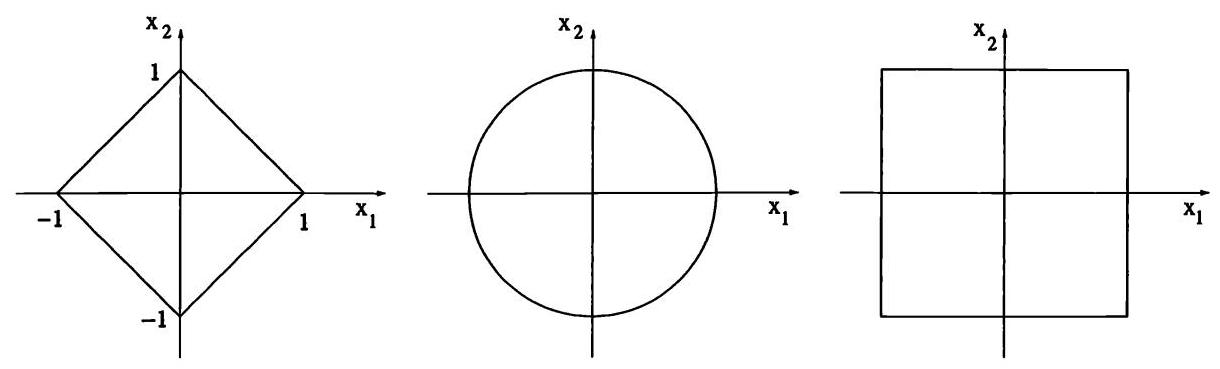
\includegraphics[width=1.0\textwidth]{images/bo_d6ik6nn7aajc739ct1l0_26_134_226_1220_369_0.jpg}
\captionof{figure}{例2.3所述的 \({\mathbb{R}}^{2}\) 中单位球，其范数分别为 \(\|  \cdot  {\| }_{1}\) (左)、 \(\|  \cdot  {\| }_{2}\) (中)和 \(\|  \cdot  {\| }_{\infty }\) (右).}
\end{center}
\hspace*{3em} 


\section{赋范空间与Banach空间的例子.}

\begin{instance}
具有欧氏范数的有限维空间 \({\mathbb{R}}^{n} = \left\{  {x = \left( {{x}_{1},\ldots ,{x}_{n}}\right) ,{x}_{i}}\right. \; \left. { \in  \mathbb{R}}\right\}\)

\begin{equation}\tag{2.2}
\| x{\| }_{2} \doteq  \sqrt{{x}_{1}^{2} + \cdots  + {x}_{n}^{2}}
\end{equation}
是实数域上的Banach空间.特别地，所有实数构成的域 \(\mathbb{R}\) 可视为一维Banach空间.此时，数 \(x \in  \mathbb{R}\) 的范数由其绝对值给出.
\end{instance}

\begin{instance}
    在空间 \({\mathbb{R}}^{n}\) 上可考虑如下替代范数

\[
\| x{\| }_{p} \doteq  {\left( {\left| {x}_{1}\right| }^{p} + \cdots  + {\left| {x}_{n}\right| }^{p}\right) }^{1/p},\;\| x{\| }_{\infty } \doteq  \mathop{\max }\limits_{{1 \leq  i \leq  n}}\left| {x}_{i}\right| .
\]

此处 \(1 \leq  p < \infty\) .这些范数中的每一个亦使 \({\mathbb{R}}^{n}\) 成为有限维Banach空间.
\end{instance}

\begin{instance}
    对任意闭有界区间 \(\left\lbrack  {a,b}\right\rbrack\) ，所有连续函数 \(f : \left\lbrack  {a,b}\right\rbrack   \mapsto  \mathbb{R}\) 构成的空间 \({\mathcal{C}}^{0}\left( \left\lbrack  {a,b}\right\rbrack  \right)\) (赋予范数

\begin{equation}\tag{2.3}
\| f{\| }_{{\mathcal{C}}^{0}} \doteq  \mathop{\max }\limits_{{x \in  \left\lbrack  {a,b}\right\rbrack  }}\left| {f\left( x\right) }\right| ,
\end{equation}
是Banach空间.
\end{instance}

\begin{instance}
    设 \(\Omega\) 为 \({\mathbb{R}}^{n}\) 的开子集.对每个 \(1 \leq  p < \infty\) ，考虑所有勒贝格可测函数 \(f : \Omega  \mapsto  \mathbb{R}\) 构成的空间 \({\mathbf{L}}^{p}\left( \Omega \right)\) ，满足 \({\int }_{\Omega }{\left| f\left( x\right) \right| }^{p}{dx} < \infty\) .此空间在范数

\begin{equation}\tag{2.4}
\| f{\| }_{{\mathbf{L}}^{p}} \doteq  {\left( {\int }_{\Omega }{\left| f\left( x\right) \right| }^{p}dx\right) }^{1/p}.
\end{equation}
下构成Banach空间.此处若两函数 \(f,\widetilde{f}\) 几乎处处相等(即 \(\operatorname{meas}\left( {\{ x \in  \Omega ;f\left( x\right)  \neq  \widetilde{f}\left( x\right) \} }\right)  = 0\) )，则视其为 \({\mathbf{L}}^{p}\left( \Omega \right)\) 中的同一元素.

类似地，所有本质有界、可测函数 \(f : \Omega  \mapsto  \mathbb{R}\) 构成的空间 \({\mathbf{L}}^{\infty }\left( \Omega \right)\) 在范数

\begin{equation}\tag{2.5}
\| f{\| }_{{\mathbf{L}}^{\infty }} \doteq  \underset{x \in  \Omega }{\operatorname{ess}\sup }\left| {f\left( x\right) }\right| .
\end{equation}
\end{instance}

\begin{instance}
    对固定 \(p \geq  1\) ，考虑所有实数序列构成的空间，其 \(p\) 次幂可求和:

\begin{equation}\tag{2.6}
{\ell }^{p} \doteq  \left\{  {\mathbf{x} = \left( {{x}_{1},{x}_{2},\ldots }\right) ;\mathop{\sum }\limits_{{k = 1}}^{\infty }{\left| {x}_{k}\right| }^{p} < \infty }\right\}
\end{equation}

此空间在范数

\begin{equation}\tag{2.7}
\| \mathbf{x}{\| }_{p} \doteq  {\left( \mathop{\sum }\limits_{{k = 1}}^{\infty }{\left| {x}_{k}\right| }^{p}\right) }^{1/p}
\end{equation}

\end{instance}
\begin{instance}
    所有有界实数序列构成的空间 \({\ell }^{\infty }\) (赋予范数

\begin{equation}\tag{2.8}
\| \mathbf{x}{\| }_{\infty } \doteq  \mathop{\sup }\limits_{{k \geq  1}}\left| {x}_{k}\right|
\end{equation}

是Banach空间.在此空间中，可考虑子空间 \({c}_{0}\) ，即所有满足 \(k \rightarrow  \infty\) 时趋于零的序列 \({\left( {x}_{k}\right) }_{k \geq  1}\) 构成的子空间.该子空间在相同范数(2.8)下亦为Banach空间.

\end{instance}

\begin{remark}
    在空间 \({\ell }^{p},1 \leq  p < \infty\) 中，考虑单位向量族(2.9)

\[
{\mathbf{e}}_{1} = \left( {1,0,0,0,\ldots }\right) ,\;{\mathbf{e}}_{2} = \left( {0,1,0,0,\ldots }\right) ,\;{\mathbf{e}}_{3} = \left( {0,0,1,0,\ldots }\right) ,\;\ldots
\]

这些向量线性无关.所有线性组合\footnote{注意，线性组合始终指有限和，而非级数.}

\begin{equation}\tag{2.10}
\operatorname{span}\left\{  {{\mathbf{e}}_{k};k \geq  1}\right\}   = \left\{  {\mathop{\sum }\limits_{{k = 1}}^{N}{\theta }_{k}{\mathbf{e}}_{k};N \geq  1,{\theta }_{k} \in  \mathbb{R}}\right\}
\end{equation}
并不等于整个空间 \({\ell }^{p}\) ，但构成 \({\ell }^{p}\) 的一个稠密子集.事实上，它由形如 \(x = \left( {{x}_{1},{x}_{2},\ldots ,{x}_{N},0,0,0,\ldots }\right)\) 且仅有有限个非零项的序列全体组成.

集合 \(\left\{  {{\mathbf{e}}_{k};k \geq  1}\right\}\) 并非 \({\ell }^{p}\) 的代数基，但提供了一个拓扑基:即每个元素 \(\mathbf{x} = \left( {{x}_{1},{x}_{2},\ldots }\right)  \in  {\ell }^{p}\) 均可表为收敛级数

\[
\mathbf{x} = \mathop{\sum }\limits_{{k = 1}}^{\infty }{x}_{k}{\mathbf{e}}_{k}
\]
\end{remark}
\begin{remark}
    在实数域或复数域上，绝对值 \(\left| \alpha \right|\) 刻画了数 \(\alpha\) 的大小.类似地，在向量空间 \(X\) 上，范数 \(\| f\|\) 可视为刻画元素 \(f \in  X\) 的大小.然而我们注意到，可在同一函数空间上采用不同的范数(从而得到不同的距离)，进而获得截然不同的收敛结果.下一例将对此加以说明.
\end{remark}

例 2.10．设 \(X\) 为区间 \(\left\lbrack  {0,1}\right\rbrack\) 上所有多项式函数构成的空间.在 \(X\) 上可考虑如下两个范数

\begin{equation}\tag{2.11}
\| f{\| }_{{\mathcal{C}}^{0}} \doteq  \mathop{\max }\limits_{{x \in  \left\lbrack  {0,1}\right\rbrack  }}\left| {f\left( x\right) }\right| ,\;\| f{\| }_{{\mathbf{L}}^{1}} \doteq  {\int }_{0}^{1}\left| {f\left( x\right) }\right| {dx}.
\end{equation}

这两个范数给出不同的收敛结果(见图 2.1.2).例如，考虑单项式序列 \({f}_{n}\left( x\right)  = {x}^{n}\) .令 \(n \rightarrow  \infty\) ，则有 \({\begin{Vmatrix}{f}_{n}\end{Vmatrix}}_{{\mathbf{L}}^{1}} \rightarrow  0\) .因此序列 \({\left( {f}_{n}\right) }_{n \geq  1}\) 在 \({\mathbf{L}}^{1}\) 范数下收敛于零(即恒等于零的函数).另一方面，对所有 \(n \geq  1\) 均有 \({\begin{Vmatrix}{f}_{n}\end{Vmatrix}}_{{\mathcal{C}}^{0}} = 1\) .就 \({\mathcal{C}}^{0}\) 范数而言，该序列并非柯西列，且无任何极限.

\begin{center}
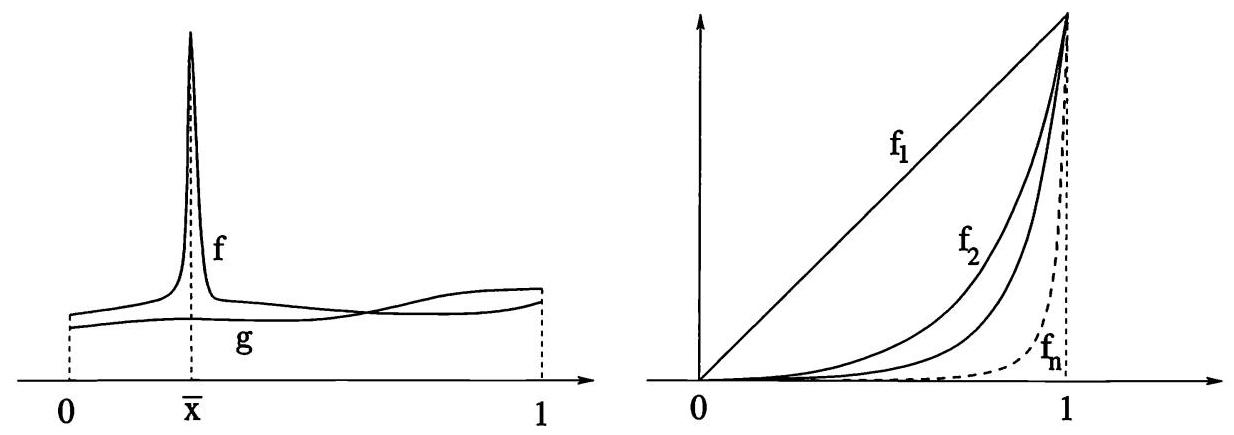
\includegraphics[width=1.0\textwidth]{images/bo_d6ik6nn7aajc739ct1l0_28_122_1102_1234_435_0.jpg}
\end{center}
\hspace*{3em} 

图 2.1.2．左:由阴影区域面积所度量的两函数 \(f,g\) 之间的 \({\mathbf{L}}^{1}\) 距离较小；但由 \(\| f - g{\| }_{{\mathcal{C}}^{0}} = \left| {f\left( \bar{x}\right)  - g\left( \bar{x}\right) }\right|\) 所度量的它们的 \({\mathcal{C}}^{0}\) 距离却很大.右:多项式序列 \({f}_{n}\left( x\right)  = {x}^{n}\) 在空间 \({\mathbf{L}}^{1}\left( \left\lbrack  {0,1}\right\rbrack  \right)\) 中收敛于零，但在空间 \({\mathcal{C}}^{0}\left( \left\lbrack  {0,1}\right\rbrack  \right)\) 中无任何极限.

\section*{2.2．线性算子}

设 \(X,Y\) 是同一标量数域 \(\mathbb{K}\) 上的赋范空间.线性算子是指从子空间 \(\operatorname{Dom}\left( \Lambda \right)  \subseteq  X\) 到 \(Y\) 的映射 \(\Lambda\) ，满足

\[
\Lambda \left( {{c}_{1}{x}_{1} + {c}_{2}{x}_{2}}\right)  = {c}_{1}\Lambda {x}_{1} + {c}_{2}\Lambda {x}_{2}\;\text{ for all }{x}_{1},{x}_{2} \in  \operatorname{Dom}\left( \Lambda \right) ,{c}_{1},{c}_{2} \in  \mathbb{K}.
\]

此处 \(\operatorname{Dom}\left( \Lambda \right)\) 是 \(\Lambda\) 的定义域. \(\Lambda\) 的值域是子空间

\[
\operatorname{Range}\left( \Lambda \right)  \doteq  \{ {\Lambda x};x \in  \operatorname{Dom}\left( \Lambda \right) \}  \subset  Y.
\]

\(\Lambda\) 的零空间(或核)是子空间

\[
\operatorname{Ker}\left( \Lambda \right)  \doteq  \{ x \in  X;{\Lambda x} = 0\}  \subseteq  X.
\]

注意， \(\Lambda\) 是单射当且仅当 \(\operatorname{Ker}\left( \Lambda \right)  = \{ 0\}\) .

接下来，考虑定义在整个空间 \(X\) 上的线性算子 \(\Lambda  : X \mapsto  Y\) ，即满足 \(\operatorname{Dom}\left( \Lambda \right)  = X\) .若 \(\Lambda\) 满足以下条件，则称其为有界的:

\begin{equation}\tag{2.12}
\| \Lambda \|  \doteq  \mathop{\sup }\limits_{{\| x\|  \leq  1}}\| {\Lambda x}\|  < \infty .
\end{equation}
\begin{theorem}[有界算子的连续性]
    线性算子 \(\Lambda  : X \mapsto  Y\) 有界当且仅当它连续.
\end{theorem}
定理 2.11()．

证明:1. 若 \(\Lambda\) 连续，则特别地，它在原点处连续.因此存在 \(\delta  > 0\) ，使得 \(\| x\|  \leq  \delta\) 蕴含 \(\| {\Lambda x}\|  \leq  1\) .由线性性，这表明

\[
\| {\Lambda x}\|  \leq  \frac{1}{\delta }\;\text{ whenever }\;\| x\|  \leq  1.
\]

故 \(\Lambda\) 有界.

2. 反之，设 \(\Lambda\) 有界，即(2.12)成立.由线性性可得

\[
\begin{Vmatrix}{\Lambda {x}_{1} - \Lambda {x}_{2}}\end{Vmatrix} = \begin{Vmatrix}{\Lambda \left( {{x}_{1} - {x}_{2}}\right) }\end{Vmatrix} = \begin{Vmatrix}{{x}_{1} - {x}_{2}}\end{Vmatrix}\begin{Vmatrix}{\Lambda \left( \frac{{x}_{1} - {x}_{2}}{\begin{Vmatrix}{x}_{1} - {x}_{2}\end{Vmatrix}}\right) }\end{Vmatrix} \leq  \begin{Vmatrix}{{x}_{1} - {x}_{2}}\end{Vmatrix}\begin{Vmatrix}\Lambda \end{Vmatrix}.
\]

故 \(\Lambda\) 一致Lipschitz连续，Lipschitz常数为 \(\| \Lambda \|\) .

若 \(X,Y\) 是同一标量域上的赋范空间，我们用 \(\mathcal{B}\left( {X;Y}\right)\) 表示从 \(X\) 到 \(Y\) 的有界线性算子空间.注意此处要求这些算子的定义域为整个空间 \(X\) .

定理2.12(有界线性算子空间):从 \(X\) 到 \(Y\) 的所有有界线性算子构成的空间 \(\mathcal{B}\left( {X;Y}\right)\) 是一个赋范空间，其范数由(2.12)定义；若 \(Y\) 是Banach空间，则 \(\mathcal{B}\left( {X;Y}\right)\) 也是Banach空间.

证明:若 \({\Lambda }_{1},{\Lambda }_{2}\) 是线性算子，且 \({\mathrm{c}}_{1},{\mathrm{c}}_{2} \in  \mathbb{K}\) ，则其线性组合定义为

\[
\left( {{\mathrm{c}}_{1}{\Lambda }_{1} + {c}_{2}{\Lambda }_{2}}\right) \left( x\right)  \doteq  {\mathrm{c}}_{1}{\Lambda }_{1}x + {\mathrm{c}}_{2}{\Lambda }_{2}x.
\]

现验证范数的性质(N1)-(N3)均成立.

1. 若 \(\Lambda  = 0\) 是零算子，则对所有 \(x \in  X\) 有 \({\Lambda x} = 0\) ，且 \(\| \Lambda \|  = 0\) .反之，若 \(\Lambda\) 不是零算子，则存在某个 \(x \neq  0\) 使得 \({\Lambda x} \neq  0\) .故 \(\Lambda \left( \frac{x}{\| x\| }\right)  = \frac{1}{\| x\| }{\Lambda x} \neq  0\) ，且(2.12)中的上确界严格为正.这证明了(N1).

2. 若 \(\alpha  \in  \mathbb{K}\) ，则(N2)由如下恒等式推出

\[
\| {\alpha \Lambda }\|  = \mathop{\sup }\limits_{{\| x\|  \leq  1}}\| {\alpha \Lambda x}\|  = \left| \alpha \right| \mathop{\sup }\limits_{{\| x\|  \leq  1}}\| {\Lambda x}\|  = \left| \alpha \right| \| \Lambda \| .
\]

3. 为验证三角不等式(N3)，对任意满足 \(\| x\|  \leq  1\) 的 \(x \in  X\) ，我们写出

\[
\begin{Vmatrix}{\left( {{\Lambda }_{1} + {\Lambda }_{2}}\right) x}\end{Vmatrix} = \begin{Vmatrix}{{\Lambda }_{1}x + {\Lambda }_{2}x}\end{Vmatrix} \leq  \begin{Vmatrix}{{\Lambda }_{1}x}\end{Vmatrix} + \begin{Vmatrix}{{\Lambda }_{2}x}\end{Vmatrix} \leq  \begin{Vmatrix}{\Lambda }_{1}\end{Vmatrix} + \begin{Vmatrix}{\Lambda }_{2}\end{Vmatrix}.
\]

对所有满足 \(\| x\|  \leq  1\) 的 \(x \in  X\) 取上确界，即得(N3).

4. 接着，假设 \(Y\) 是Banach空间.需证 \(\mathcal{B}\left( {X;Y}\right)\) 完备.设 \({\left( {\Lambda }_{n}\right) }_{n \geq  1}\) 是一列有界线性算子的Cauchy列.对每个 \(x \in  X\) ，这蕴含

\[
\mathop{\limsup }\limits_{{m,n \rightarrow  \infty }}\begin{Vmatrix}{{\Lambda }_{m}x - {\Lambda }_{n}x}\end{Vmatrix} \leq  \mathop{\limsup }\limits_{{m,n \rightarrow  \infty }}\begin{Vmatrix}{{\Lambda }_{m} - {\Lambda }_{n}}\end{Vmatrix}\| x\|  = 0.
\]

因此点列 \({\left( {\Lambda }_{n}x\right) }_{n \geq  1}\) 在 \(Y\) 中为Cauchy列.由于 \(Y\) 完备，该列有唯一极限，记为 \({\Lambda x}\) .

因每个 \({\Lambda }_{n}\) 均为线性算子，显然 \(\Lambda\) 亦为线性算子.我们断言 \(\Lambda\) 亦有界(从而连续).由假设，可选取足够大的 \(N\) 使得

\[
\begin{Vmatrix}{{\Lambda }_{k} - {\Lambda }_{N}}\end{Vmatrix} \leq  1\;\text{ for all }k \geq  N.
\]

因此，对任意满足 \(\| x\|  \leq  1\) 的 \(x \in  X\) ，均有

\[
\| {\Lambda x}\|  = \mathop{\lim }\limits_{{k \rightarrow  \infty }}\begin{Vmatrix}{{\Lambda }_{k}x}\end{Vmatrix} \leq  \begin{Vmatrix}{{\Lambda }_{N}x}\end{Vmatrix} + \mathop{\limsup }\limits_{{k \rightarrow  \infty }}\begin{Vmatrix}{{\Lambda }_{k} - {\Lambda }_{N}}\end{Vmatrix}\| x\|  \leq  \begin{Vmatrix}{\Lambda }_{N}\end{Vmatrix} + 1.
\]

由于 \(x\) 是单位球中的任意一点，这证明极限算子 \(\Lambda\) 有界，从而 \(\Lambda  \in  \mathcal{B}\left( {X;Y}\right)\) .

\section*{2.2.1. 线性算子示例.}

例2.13(矩阵作为线性算子).每个 \(n \times  m\) 矩阵 \(A = \left( {a}_{ij}\right)\) 确定一个由下式定义的有界线性算子 \(\Lambda  : {\mathbb{R}}^{m} \mapsto  {\mathbb{R}}^{n}\) :

\[
\Lambda \left( {{x}_{1},\ldots ,{x}_{m}}\right)  = \left( {{y}_{1},\ldots ,{y}_{n}}\right) ,\;\text{ with }\;{y}_{i} \doteq  \mathop{\sum }\limits_{{j = 1}}^{m}{a}_{ij}{x}_{j}.
\]

例2.14(序列空间上的对角算子).设 \(1 \leq  p \leq  \infty\) ，并考虑所有实数序列 \(\mathbf{x} = \left( {{x}_{1},{x}_{2},\ldots }\right)\) 构成的空间 \(X = {\ell }^{p}\) ，其范数按(2.7)或(2.8)式定义.设 \(\left( {{\lambda }_{1},{\lambda }_{2},\ldots }\right)\) 为任意实数序列，并将算子 \(\Lambda  : X \mapsto  X\) 定义为:

\begin{equation}\tag{2.13}
\Lambda \left( {{x}_{1},{x}_{2},{x}_{3},\ldots }\right)  \doteq  \left( {{\lambda }_{1}{x}_{1},{\lambda }_{2}{x}_{2},{\lambda }_{3}{x}_{3},\ldots }\right) .
\end{equation}

参照(2.9)式中单位向量基 \(\left\{  {{\mathbf{e}}_{1},{\mathbf{e}}_{2},\ldots }\right\}\) ，可将 \(\Lambda\) 视作一个无穷矩阵:

\[
\left( \begin{matrix} {\lambda }_{1} & 0 & & & \\  0 & {\lambda }_{2} & & & \\   & & {\lambda }_{3} & & \\   & & & &  \end{matrix}\right)
\]

其对角线元素为 \({\lambda }_{1},{\lambda }_{2},\ldots\) ，其余位置均为0.此时我们分两种情形.

(i) 若序列 \({\left( {\lambda }_{k}\right) }_{k \geq  1}\) 有界，则算子 \(\Lambda\) 有界，其范数为

\begin{equation}\tag{2.14}
\| \Lambda \|  = \mathop{\sup }\limits_{k}\left| {\lambda }_{k}\right|
\end{equation}

(ii) 若序列 \({\left( {\lambda }_{k}\right) }_{k \geq  1}\) 无界，则算子 \(\Lambda\) 无界，其定义域

\[
\operatorname{Dom}\left( \Lambda \right)  = \left\{  {x \in  {\ell }^{p};{\Lambda x} \in  {\ell }^{p}}\right\}
\]

是一个向量子空间，且严格包含于 \({\ell }^{p}\) 中.

例2.15(微分算子).考虑开区间 \(I = \rbrack 0,\pi \lbrack\) ，令 \(X = \mathcal{B}C\left( I\right)\) 为 \(I\) 上所有有界连续实值函数构成的空间，其范数为

\[
\| f\|  = \mathop{\sup }\limits_{{0 < x < \pi }}\left| {f\left( x\right) }\right| .
\]

\({\Lambda f} = {f}^{\prime }\) 微分算子显然是 \(X\) 上的线性算子.为说明该算子无界，考虑函数列 \({f}_{k}\left( x\right)  = \sin {kx}\) .此时 \({f}_{k}^{\prime }\left( x\right)  = k\cos {kx}\) ，故

\[
\begin{Vmatrix}{f}_{k}\end{Vmatrix} = 1,\;\begin{Vmatrix}{\Lambda {f}_{k}}\end{Vmatrix} = k\;\text{ for all }k \geq  1.
\]

该微分算子的定义域 \(\operatorname{Dom}\left( \Lambda \right)\) 是所有处处可微、且导数有界连续的有界连续函数 \(f : I \mapsto  \mathbb{R}\) 构成的空间.这是 \(\mathcal{B}C\left( I\right)\) 的一个真子空间.

例2.16( \({\mathbf{L}}^{p}\left( \mathbb{R}\right)\) 上的移位算子).令 \(1 \leq  p \leq  \infty\) .任取 \(a \in  \mathbb{R}\) .对任意函数 \(f \in  {\mathbf{L}}^{p}\left( \mathbb{R}\right)\) ，定义 \(\left( {{\Lambda }_{a}f}\right) \left( x\right)  \doteq  f\left( {x - a}\right)\) .显然 \(\| {\Lambda f}{\| }_{{\mathbf{L}}^{p}} = \| f{\| }_{{\mathbf{L}}^{p}}\) .因此 \({\Lambda }_{a} : {\mathbf{L}}^{p} \mapsto  {\mathbf{L}}^{p}\) 是有界线性算子，其范数为 \(\begin{Vmatrix}{\Lambda }_{a}\end{Vmatrix} = 1\) .注意，算子 \({\Lambda }_{a}\) 是一一映射且满射.

例2.17( \({\ell }^{p}\) 上的移位算子).令 \(1 \leq  p \leq  \infty\) .定义算子 \({\Lambda }_{ + } : {\ell }^{p} \mapsto  {\ell }^{p}\) 与 \({\Lambda }_{ - } : {\ell }^{p} \mapsto  {\ell }^{p}\) 如下:

\[
{\Lambda }_{ + }\left( {{x}_{1},{x}_{2},{x}_{3},\ldots }\right)  \doteq  \left( {0,{x}_{1},{x}_{2},\ldots }\right)
\]

\[
{\Lambda }_{ - }\left( {{x}_{1},{x}_{2},{x}_{3},\ldots }\right)  \doteq  \left( {{x}_{2},{x}_{3},{x}_{4},\ldots }\right)
\]

注意到它们均为线性连续算子，且满足 \(\begin{Vmatrix}{\Lambda }_{ + }\end{Vmatrix} = \begin{Vmatrix}{\Lambda }_{ - }\end{Vmatrix} = 1\) .此外， \({\Lambda }_{ + }\) 是一一映射但非满射，而 \({\Lambda }_{ - }\) 是满射但非一一映射.

例2.18(乘法算子).设 \(\Omega  \subset  {\mathbb{R}}^{n}\) ，且 \(g : \Omega  \mapsto  \mathbb{R}\) 为一有界可测函数.对任意 \(1 \leq  p \leq  \infty\) ，在空间 \({\mathbf{L}}^{p}\left( \Omega \right)\) 上考虑乘法算子: \(\left( {{M}_{g}f}\right) \left( x\right)  \doteq  g\left( x\right) f\left( x\right)\) .该算子连续，其范数为

\begin{equation}\tag{2.15}
\begin{Vmatrix}{M}_{g}\end{Vmatrix} \doteq  \mathop{\sup }\limits_{{\| f{\| }_{{\mathbf{L}}^{p}} \leq  1}}\| {gf}{\| }_{{\mathbf{L}}^{p}} = \| g{\| }_{{\mathbf{L}}^{\infty }}.
\end{equation}

例2.19(积分算子).设 \(a < b\) ，并考虑定义在闭区间 \(\left\lbrack  {a,b}\right\rbrack\) 上的实值连续函数空间 \(X = {\mathcal{C}}^{0}\left( \left\lbrack  {a,b}\right\rbrack  \right)\) .考虑积分算子

\[
\left( {\Lambda f}\right) \left( x\right)  \doteq  {\int }_{a}^{x}f\left( y\right) {dy}.
\]

则 \(\Lambda  : X \mapsto  X\) 是有界线性算子.事实上，

\[
\left| {\left( {\Lambda f}\right) \left( x\right) }\right| \; = \;\left| {{\int }_{a}^{x}f\left( y\right) \;{dy}}\right| \; \leq  \;{\int }_{a}^{x}\left| {f\left( y\right) }\right| \;{dy}\; \leq  \;\left( {b - a}\right)  \cdot  \mathop{\max }\limits_{{x \in  \left\lbrack  {a,b}\right\rbrack  }}\left| {f\left( x\right) }\right| .
\]

因此 \(\| {\Lambda f}\|  \leq  \left( {b - a}\right) \| f\|\) 且 \(\| \Lambda \|  \leq  \left( {b - a}\right)\) .

\section*{2.3 有限维空间}

我们称同一向量空间 \(X\) 上的两个范数 \(\|  \cdot  {\| }_{\diamond }\) 与 \(\|  \cdot  {\| }_{\diamond }\) 等价，若存在常数 \(C \geq  1\) ，使得

\begin{equation}\tag{2.16}
\frac{1}{C}\| x{\| }_{\diamond } \leq  \| x{\| }_{\spadesuit } \leq  C\| x{\| }_{\diamond }\;\text{ for all }x \in  X.
\end{equation}

等价范数在 \(X\) 上给出相同的柯西列和相同的拓扑.一般而言，无限维空间 \(X\) 可具有许多互不等价的范数.如例2.10所示，在单实变量多项式全体构成的空间上， \({\mathbf{L}}^{1}\) 范数与(2.11)式中定义的 \({\mathcal{C}}^{0}\) 范数并不等价.

接下来的结果表明:对任意有限维向量空间 \(X\) ，其所有范数均等价.事实上，每个维数为 \(N\) 的有限维赋范空间均与欧几里得空间 \({\mathbb{K}}^{N}\) 等价.我们回顾:向量 \(\alpha  = \left( {{\alpha }_{1},\ldots ,{\alpha }_{N}}\right)  \in  {\mathbb{K}}^{N}\) 的欧几里得范数为 \(\| \alpha \|  \doteq  \sqrt{\mathop{\sum }\limits_{k}{\left| {\alpha }_{k}\right| }^{2}}\) .

定理2.20(有限维赋范空间同胚于 \({\mathbb{K}}^{N}\) ).设 \(X\) 为定义在实数或复数域 \(\mathbb{K}\) 上的有限维赋范空间， \(\mathcal{B} = \left\{  {{u}_{1},{u}_{2},\ldots ,{u}_{N}}\right\}\) 为其一组基.则

(i) \(X\) 完备，因而为Banach空间.

(ii) 对每个 \(\alpha  = \left( {{\alpha }_{1},{\alpha }_{2},\ldots ,{\alpha }_{N}}\right)  \in  {\mathbb{K}}^{N}\) ，定义

\begin{equation}\tag{2.17}
{\Lambda \alpha } \doteq  {\alpha }_{1}{u}_{1} + {\alpha }_{2}{u}_{2} + \cdots  + {\alpha }_{N}{u}_{N}.
\end{equation}

则线性算子 \(\Lambda  : {\mathbb{K}}^{N} \mapsto  X\) 是双射且有界的.此外，其逆算子 \({\Lambda }^{-1} : X \mapsto  {\mathbb{K}}^{N}\) 亦有界.

证明.1. \(\left\{  {{u}_{1},\ldots ,{u}_{N}}\right\}\) 为基这一事实意味着 \(\Lambda\) 是单射且满射，故逆算子 \({\Lambda }^{-1} : X \mapsto  {\mathbb{K}}^{N}\) 良定义.

2. 将

\[
\| {\Lambda \alpha }\|  \leq  \mathop{\sum }\limits_{{k = 1}}^{N}\begin{Vmatrix}{{\alpha }_{k}{u}_{k}}\end{Vmatrix} \leq  \| \alpha \| \mathop{\sum }\limits_{{k = 1}}^{N}\begin{Vmatrix}{u}_{k}\end{Vmatrix},
\]

展开可见， \(\Lambda  : {\mathbb{K}}^{N} \mapsto  X\) 为有界线性算子，因而连续.

3. 我们断言 \({\Lambda }^{-1}\) 也有界.否则，存在 \(X\) 中的一个序列 \({\left( {x}_{n}\right) }_{n \geq  1}\) ，使得对每个 \(n\) 均有 \(\begin{Vmatrix}{x}_{n}\end{Vmatrix} \leq  1\) ，且

\[
\begin{Vmatrix}{{\Lambda }^{-1}{x}_{n}}\end{Vmatrix} \rightarrow  \infty \;\text{ as }n \rightarrow  \infty .
\]

考虑归一化向量

\[
{\beta }_{n} \doteq  \frac{{\Lambda }^{-1}{x}_{n}}{\begin{Vmatrix}{\Lambda }^{-1}{x}_{n}\end{Vmatrix}} \in  {\mathbb{K}}^{N}.
\]

于是 \(\begin{Vmatrix}{\beta }_{n}\end{Vmatrix} = 1\) 且 \(\Lambda {\beta }_{n} \rightarrow  0\) 当 \(n \rightarrow  \infty\) 时成立.由于 \({\left( {\beta }_{n}\right) }_{n \geq  1}\) 是欧几里得空间 \({\mathbb{K}}^{N}\) 中的有界序列，故存在收敛子列，记为 \({\beta }_{{n}_{k}} \rightarrow  \beta  \in  {\mathbb{K}}^{N}\) .显然

\[
\| \beta \| \; = \;\mathop{\lim }\limits_{{k \rightarrow  \infty }}\begin{Vmatrix}{\beta }_{{n}_{k}}\end{Vmatrix}\; = \;1,\;{\Lambda \beta }\; = \;\mathop{\lim }\limits_{{k \rightarrow  \infty }}\Lambda {\beta }_{{n}_{k}}\; = \;\mathop{\lim }\limits_{{k \rightarrow  \infty }}\frac{{x}_{{k}_{n}}}{\begin{Vmatrix}{\Lambda }^{-1}{x}_{{k}_{n}}\end{Vmatrix}}\; = \;0\;,
\]

因为 \(\Lambda\) 连续.这与 \(\Lambda\) 是单射相矛盾.因此我们得出结论: \({\Lambda }^{-1}\) 有界，从而连续.这就证明了 (ii).

4. 为证范数为 \(\|  \cdot  \|\) 的 \(X\) 完备，设 \({\left( {x}_{n}\right) }_{n \geq  1}\) 是 \(X\) 中的柯西序列.则 \({\Lambda }^{-1}{x}_{n}\) 在 \({\mathbb{K}}^{N}\) 中构成柯西序列；由于 \({\mathbb{K}}^{N}\) 完备，该序列收敛于某点 \(\beta  \in  {\mathbb{K}}^{N}\) .又因 \(\Lambda\) 连续，故序列 \({x}_{n}\) 收敛于 \({\Lambda \beta }\) .

推论 2.21. 在有限维空间中，所有范数均等价.

证明. 设 \(\|  \cdot  {\| }_{\diamond }\) 和 \(\|  \cdot  {\| }_{\diamond }\) 是有限维向量空间 \(X\) 上的任意两个范数.令 \(\mathcal{B} = \left\{  {{u}_{1},\ldots ,{u}_{N}}\right\}\) 是 \(X\) 的一组基，并如 (2.17) 式定义线性映射 \(\Lambda  : {\mathbb{K}}^{N} \mapsto  X\) .由前述定理， \(\Lambda\) 与 \({\Lambda }^{-1}\) 均为有界线性算子(在 \(X\) 的这两种范数下).因此存在常数 \({C}^{\prime },{C}^{\prime \prime }\) ，使得

\[
\frac{1}{{C}^{\prime }}\begin{Vmatrix}{{\Lambda }^{-1}x}\end{Vmatrix} \leq  \| x{\| }_{\diamond } \leq  {C}^{\prime }\begin{Vmatrix}{{\Lambda }^{-1}x}\end{Vmatrix}
\]

\[
\frac{1}{{C}^{\prime \prime }}\begin{Vmatrix}{{\Lambda }^{-1}x}\end{Vmatrix} \leq  \| x{\| }_{\spadesuit } \leq  {C}^{\prime \prime }\begin{Vmatrix}{{\Lambda }^{-1}x}\end{Vmatrix},
\]

对所有 \(x \in  X\) 成立.这即推出 (2.16) 式.

波尔查诺-Weierstrass经典定理指出: \({\mathbb{R}}^{N}\) 中每个有界序列都存在收敛子列.下一个定理表明，这一紧性性质对所有有限维赋范空间成立，而对所有无限维赋范空间均不成立.

定理 2.22(局部紧的赋范空间必为有限维). 设 \(X\) 是一个赋范空间.以下命题等价:

(i) \(X\) 是有限维的.

(ii) 闭单位球 \({B}_{1} \doteq  \overline{B\left( {0,1}\right) } = \{ x \in  X;\| x\|  \leq  1\}\) 是紧的.

\begin{center}
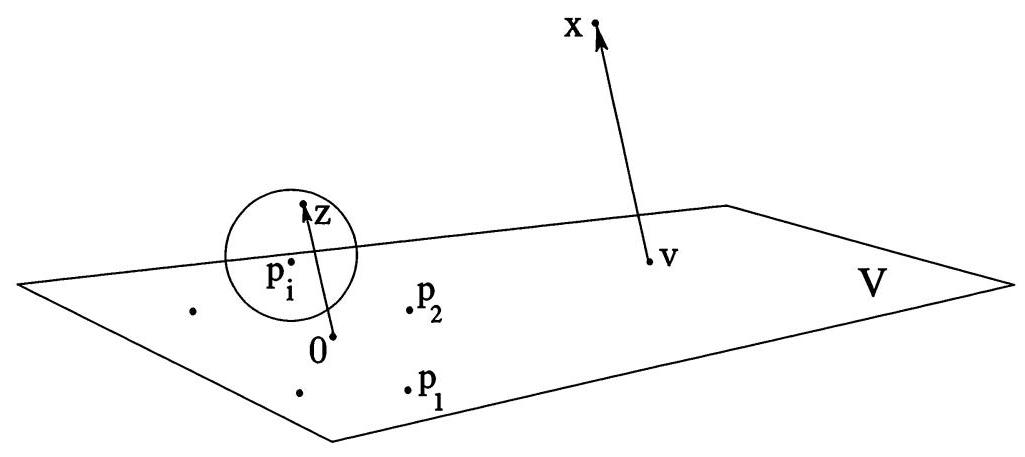
\includegraphics[width=0.9\textwidth]{images/bo_d6ik6nn7aajc739ct1l0_34_221_1328_1025_457_0.jpg}
\end{center}
\hspace*{3em} 

图 2.3.1. 用于证明定理 2.22 的构造.

证明:(i) \(\Rightarrow\) .(ii) 设 \(X\) 的维数为 \(N\) .则由定理 2.20，存在一个具有有界逆的线性同胚映射 \(\Lambda  : {\mathbb{K}}^{N} \mapsto  X\) .由于单位球 \({B}_{1} \subset  X\) 是闭且有界的，故 \(K \doteq \; {\Lambda }^{-1}\left( {B}_{1}\right)  \subset  {\mathbb{K}}^{N}\) 同样闭且有界.由波尔查诺-Weierstrass定理，闭有集 \(K\) 是紧的.而 \({B}_{1} = \Lambda \left( K\right)\) 作为紧集的连续像，亦为紧集.

(ii) \(\Rightarrow\) (i).假设闭单位球 \({B}_{1} \subset  X\) 是紧的，则其是列紧的，可用有限个以点 \({p}_{i},i = 1,\ldots ,n\) 为中心、半径为 \(1/2\) 的开球 \(B\left( {{p}_{i},1/2}\right)\) 覆盖.考虑有限维子空间 \(V = \operatorname{span}\left\{  {{p}_{1},\ldots ,{p}_{n}}\right\}\) (见图 2.3.1).注意 \(V\) 在 \(X\) 中是闭的，因为根据定理 2.20，每个有限维赋范空间都是完备的.

我们断言 \(V = X\) ，从而 \(X\) 本身是有限维的.否则，可找到一点 \(x \in  X \setminus  V\) .令 \(\rho  \doteq  d\left( {x,V}\right)  \doteq  \mathop{\inf }\limits_{{y \in  V}}\| y - x\|\) .注意到 \(\rho  > 0\) ，因为 \(V\) 是闭的.因此存在一点 \(v \in  V\) ，使得

\begin{equation}\tag{2.18}
\rho  \leq  \| x - v\|  \leq  \frac{3}{2}\rho .
\end{equation}

考虑单位向量

\[
z \doteq  \frac{x - v}{\| x - v\| } \in  {B}_{1}.
\]

由构造可知，存在一点 \({p}_{i} \in  {B}_{1}\) ，使得 \(\begin{Vmatrix}{z - {p}_{i}}\end{Vmatrix} < \frac{1}{2}\) .于是我们有

\[
x = v + \| x - v\| z = v + \| x - v\| {p}_{i} + \| x - v\| \left( {z - {p}_{i}}\right) .
\]

由于 \(v + \| x - v\| {p}_{i} \in  V\) ，必有

\[
\| x - v\| \begin{Vmatrix}{z - {p}_{i}}\end{Vmatrix} \geq  d\left( {x,V}\right)  \geq  \rho .
\]

故 \(\| x - v\|  \geq  {2\rho }\) ，与 (2.18) 矛盾.这表明 \(X = V\) ，证毕.

\section*{2.4. 半范数与Fr空间}

为引出半范数的概念，我们注意到:对某些函数空间而言，并不存在定义范数的自然方式.

例 2.23.考虑开区间 ] \(0,1\lbrack\) 上所有连续(可能无界)函数构成的空间 \(X \doteq  \mathcal{C}\left( {\rbrack 0,1\lbrack }\right)\) .若定义

\[
p\left( f\right)  \doteq  \mathop{\sup }\limits_{{0 < x < 1}}\left| {f\left( x\right) }\right| ,
\]

则该式不能在整个空间 \(X\) 上给出一个范数.事实上，只要 \(f\) 无界，右端即取值为 \(+ \infty\) .

另一方面，对任意闭子区间 \(\left\lbrack  {a,b}\right\rbrack   \subset  \rbrack 0,1\lbrack\) ，“半范数”

\begin{equation}\tag{2.19}
{p}^{a,b}\left( f\right)  \doteq  \mathop{\max }\limits_{{x \in  \left\lbrack  {a,b}\right\rbrack  }}\left| {f\left( x\right) }\right|
\end{equation}

恒为一良定义的实数.注意，式 (2.19) 中的泛函不满足范数的所有要求，因为存在函数 \(f \in  \mathcal{C}\left( {\rbrack 0,1\lbrack }\right)\) 在 \(\left\lbrack  {a,b}\right\rbrack\) 上恒为零但并非恒等于零；此时 \({p}^{a,b}\left( f\right)  = 0\) 而 \(f \neq  0\) .

设 \(X\) 是域 \(\mathbb{K}\) 上的一个向量空间.实值映射 \(x \mapsto  p\left( x\right)\) 称为 \(X\) 上的一个半范数，若其满足如下性质:

(SN1) 对每个 \(x \in  X\) ，有 \(p\left( x\right)  \geq  0\) .

(SN2) 对每个 \(x \in  X\) 和 \(\lambda  \in  \mathbb{K}\) ，有 \(p\left( {\lambda x}\right)  = \left| \lambda \right| p\left( x\right)\) .

(SN3) 对每个 \(x,y \in  X,p\left( {x + y}\right)  \leq  p\left( x\right)  + p\left( y\right)\) .

注意:(SN2)-(SN3) 与范数定义中的完全相同，唯一区别在于 (SN1) 中不要求严格正性条件.换言之，我们允许 \(p\left( x\right)  = 0\) ，即使 \(x \neq  0\) .

若 \(p\left( \cdot \right)\) 是一个半范数，则通过设定 \(d\left( {x,y}\right)  \doteq  p\left( {x - y}\right)\) ，我们并不能保证在空间 \(X\) 上得到一个距离.事实上，即使 \(x \neq  y\) ，也可能有 \(d\left( {x,y}\right)  = \; p\left( {x - y}\right)  = 0\) .然而，存在一些有趣的情形:可通过不止一个、而是可数个半范数来构造距离.

我们称 \(X\) 上的一列半范数 \({\left( {p}_{k}\right) }_{k \geq  1}\) 是分离的，如果对每个满足 \(x \neq  0\) 的 \(x \in  X\) ，均存在至少一个指标 \(k\) ，使得 \({p}_{k}\left( x\right)  > 0\) .

引理 2.24(由半范数生成的距离).设 \({\left( {p}_{k}\right) }_{k \geq  1}\) 是向量空间 \(X\) 上的一列分离半范数.则

\begin{equation}\tag{2.20}
d\left( {x,y}\right)  \doteq  \mathop{\sum }\limits_{{k = 1}}^{\infty }{2}^{-k}\frac{{p}_{k}\left( {x - y}\right) }{1 + {p}_{k}\left( {x - y}\right) }
\end{equation}

在 \(X\) 上定义了一个距离.

证明.恒等式

\[
d\left( {x,x}\right)  = 0,\;d\left( {x,y}\right)  = d\left( {y,x}\right)
\]

是 (SN2) 的直接推论.序列 \(\left( {p}_{k}\right)\) 的分离性保证了只要 \(x \neq  y\) ，就有 \(d\left( {x,y}\right)  > 0\) .

为证三角不等式，注意到若 \(a,b,c \geq  0\) 且 \(c \leq \; a + b\) ，则

\[
\frac{c}{1 + c} \leq  \frac{a + b}{1 + a + b} \leq  \frac{a}{1 + a} + \frac{b}{1 + b}
\]

因为函数 \(s \mapsto  \frac{s}{1 + s}\) 是递增且向下凹的.由 (SN3)，可将上述不等式用于 \(a = {p}_{k}\left( {x - y}\right) ,b = {p}_{k}\left( {y - z}\right) ,c = {p}_{k}\left( {x - z}\right)\) ，得

\[
d\left( {x,z}\right)  = \mathop{\sum }\limits_{{k = 1}}^{\infty }{2}^{-k}\frac{{p}_{k}\left( {x - z}\right) }{1 + {p}_{k}\left( {x - z}\right) }
\]

\[
\leq  \mathop{\sum }\limits_{{k = 1}}^{\infty }{2}^{-k}\left( {\frac{{p}_{k}\left( {x - y}\right) }{1 + {p}_{k}\left( {x - y}\right) } + \frac{{p}_{k}\left( {y - z}\right) }{1 + {p}_{k}\left( {y - z}\right) }}\right)
\]

\[
= d\left( {x,y}\right)  + d\left( {y,z}\right) .
\]

这证明了 \(d\left( {\cdot , \cdot  }\right)\) 确实是一个距离.

由定义可知，距离 (2.20) 在平移下不变，即

\[
d\left( {x,y}\right)  = d\left( {x + z,y + z}\right) \;\text{ for all }x,y,z \in  X.
\]

若向量空间 \(X\) 关于距离 (2.20) 构成完备度量空间，则称 \(X\) 为 Fréchet 空间.

例 2.25.设 \(\Omega  \subseteq  {\mathbb{R}}^{n}\) 为任意开集，其边界为 \(\partial \Omega\) .则所有(可能无界)连续函数 \(f : \Omega  \mapsto  \mathbb{R}\) 构成的空间 \(\mathcal{C}\left( \Omega \right)\) 并无自然范数.但可如下赋予其 Fréchet 空间结构:对每个 \(k \geq  1\) ，考虑紧子集(图 2.4.1)

\begin{equation}\tag{2.21}
{A}_{k} \doteq  \left\{  {x \in  \Omega ;\left| x\right|  \leq  k,d\left( {x,\partial \Omega }\right)  \leq  {k}^{-1}}\right\}  .
\end{equation}

定义半范数

\begin{equation}\tag{2.22}
{p}_{k}\left( f\right)  \doteq  \mathop{\max }\limits_{{x \in  {A}_{k}}}\left| {f\left( x\right) }\right|
\end{equation}

并令 \(d\left( {\cdot , \cdot  }\right)\) 为如(2.20)式所定义的相应距离.

\begin{center}
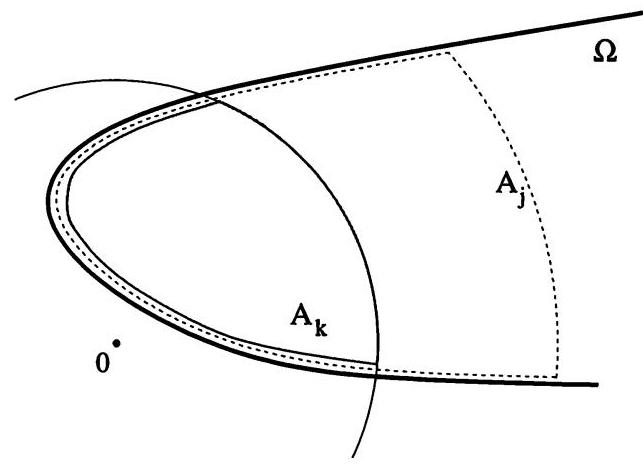
\includegraphics[width=0.6\textwidth]{images/bo_d6ik6nn7aajc739ct1l0_37_413_1667_643_469_0.jpg}
\end{center}
\hspace*{3em} 

图2.4.1:紧子集 \({A}_{k} \subset  \Omega\) .

我们证明:配备上述距离的 \(\mathcal{C}\left( \Omega \right)\) 是一个完备度量空间，因而是一个Fréchet空间.设 \({\left( {f}_{j}\right) }_{j \geq  1}\) 是一个Cauchy列.对每个 \(k\) ，这蕴含

\begin{equation}\tag{2.23}
\mathop{\limsup }\limits_{{i,j \rightarrow  \infty }}{p}_{k}\left( {{f}_{i} - {f}_{j}}\right)  = \mathop{\limsup }\limits_{{i,j \rightarrow  \infty }}\mathop{\sup }\limits_{{x \in  {A}_{k}}}\left| {{f}_{i}\left( x\right)  - {f}_{j}\left( x\right) }\right|  = 0.
\end{equation}

由于每一点 \(x \in  \Omega\) 都包含于某个集合 \({A}_{k}\) 中，由(2.23)式可知序列 \({f}_{j}\left( x\right)\) 是Cauchy列，从而收敛于某个极限 \(f\left( x\right)\) .更一般地，每个紧子集 \(K \subset  \Omega\) 都包含于某个集合 \({A}_{k}\) 中.再次由(2.23)式可知， \({f}_{j} \rightarrow  f\) 的收敛在 \(\Omega\) 的每个紧子集上是一致的，故极限 \(f\) 连续.

接下来只需证明 \(d\left( {{f}_{j},f}\right)  \rightarrow  0\) 当 \(j \rightarrow  \infty\) .对任意固定的 \(m \geq  1\) ，利用 \({f}_{j} \rightarrow  f\) 在紧集 \({A}_{m}\) 上一致收敛这一事实，可得

\[
\mathop{\limsup }\limits_{{j \rightarrow  \infty }}d\left( {{f}_{j},f}\right)
\]

\[
\leq  \mathop{\limsup }\limits_{{j \rightarrow  \infty }}\mathop{\sum }\limits_{{k = 1}}^{m}{2}^{-k}\frac{{p}_{k}\left( {{f}_{j} - f}\right) }{1 + {p}_{k}\left( {{f}_{j} - f}\right) } + \mathop{\limsup }\limits_{{j \rightarrow  \infty }}\mathop{\sum }\limits_{{k = m + 1}}^{\infty }{2}^{-k}\frac{{p}_{k}\left( {{f}_{j} - f}\right) }{1 + {p}_{k}\left( {{f}_{j} - f}\right) }
\]

\[
\leq  0 + {2}^{-m}\text{ . }
\]

由于 \(m\) 是任意的，收敛性得证.

例2.26(空间 \({\mathbf{L}}_{\text{ loc }}^{p}\) ).与前一例类似，设 \(\Omega  \subseteq  {\mathbb{R}}^{n}\) 为开集.若开集 \({\Omega }^{\prime }\) 的闭包 \({\overline{\Omega }}^{\prime }\) 是 \(\Omega\) 的紧子集，则称 \({\Omega }^{\prime }\) 紧含于 \(\Omega\) ，记作 \({\Omega }^{\prime } \subset   \subset  \Omega\) .

对 \(p \in  \left\lbrack  {1,\infty \left\lbrack  \right. }\right.\) ，定义 \({\mathbf{L}}_{\text{ loc }}^{p}\left( \Omega \right)\) 为所有可测函数 \(f\) 构成的空间，使得对每个紧含于 \(\Omega\) 的开集 \({\Omega }^{\prime }\) 均有 \({\int }_{{\Omega }^{\prime }}{\left| f\right| }^{p}{dx} < \infty\) .该空间未赋予自然范数.然而，对每个 \(k \geq  1\) ，可考虑半范数

\begin{equation}\tag{2.24}
{p}_{k}\left( f\right)  \doteq  {\left( {\int }_{{A}_{k}}{\left| f\right| }^{p}dx\right) }^{1/p} = \| f{\| }_{{\mathbf{L}}^{p}\left( {A}_{k}\right) },
\end{equation}

其中 \({A}_{k}\) 是(2.21)式中定义的集合.相应的距离(2.20)使 \({\mathbf{L}}_{\text{ loc }}^{p}\left( \Omega \right)\) 成为一个Fréchet空间.

\section*{2.5 扩张定理}

设 \(X\) 是域 \(\mathbb{K}\) 上的向量空间.线性映射 \(F : X \mapsto  \mathbb{K}\) 称为 \(X\) 上的线性泛函.本节的最终目标是证明存在大量连续线性泛函.为此，我们首先证明一个扩张定理:给定定义在子空间 \(\mathbb{K}\) 上的线性泛函

\(f : V \mapsto  \mathbb{K}\) 定义在子空间 \(V \subset  X\) 上，可将其延拓为定义在整个空间上的泛函 \(F : X \mapsto  \mathbb{K}\) ，同时保持某些附加性质.

以下考虑实数域上的向量空间 \(X\) ，并设 \(p : X \mapsto  \mathbb{R}\) 是满足如下条件的函数:

\[
\text{ ) }p\left( {x + y}\right)  \leq  p\left( x\right)  + p\left( y\right) ,\;p\left( {tx}\right)  = {tp}\left( x\right) \text{ for all }x,y \in  X,t \geq  0\text{ . }
\]

注2.27:若 \(X\) 是赋范空间，则对任意 \(\kappa  > 0\) ，函数 \(p\left( x\right)  = \kappa \| x\|\) 均满足上述性质.更一般地，任一半范数也满足(2.25)式.

注意到(2.25)式表明函数 \(p\) 是凸的.事实上

\[
p\left( {{\theta x} + \left( {1 - \theta }\right) y}\right)  \leq  p\left( {\theta x}\right)  + p\left( {\left( {1 - \theta }\right) y}\right)  = {\theta p}\left( x\right)  + \left( {1 - \theta }\right) p\left( y\right)
\]

对所有 \(x,y \in  X,\theta  \in  \left\lbrack  {0,1}\right\rbrack\) 成立.然而，与半范数相比，此处我们还允许 \(p\left( x\right)  < 0\) .此外，我们并不要求 \(p\) 关于原点对称.换言之，完全可能有 \(p\left( x\right)  \neq  p\left( {-x}\right)\) .

例2.28.设 \(X\) 为赋范空间， \(\Omega  \subset  X\) 为包含原点的有界开凸集.则泛函

\begin{equation}\tag{2.26}
p\left( x\right)  \doteq  \inf \{ \lambda  \geq  0;x \in  {\lambda \Omega }\}
\end{equation}

满足假设(2.25).

定理2.29(哈恩-Banach延拓定理).设 \(X\) 为实数域上的向量空间， \(p : X \mapsto  \mathbb{R}\) 为具有性质(2.25)的映射.考虑子空间 \(V \subseteq  X\) ，并设 \(f : V \mapsto  \mathbb{R}\) 为满足

\begin{equation}\tag{2.27}
f\left( x\right)  \leq  p\left( x\right) \;\text{ for all }x \in  V.
\end{equation}

的线性泛函.则存在线性泛函 \(F : X \mapsto  \mathbb{R}\) ，使得对所有 \(x \in  V\) 有 \(F\left( x\right)  = f\left( x\right)\) ，且

\begin{equation}\tag{2.28}
- p\left( {-x}\right)  \leq  F\left( x\right)  \leq  p\left( x\right) \;\text{ for all }x \in  X.
\end{equation}

证明.1. 若 \(V = X\) ，注意到 \(f\left( x\right)  =  - f\left( {-x}\right)  \geq   - p\left( {-x}\right)\) ，结论显然.若 \(V \neq  X\) ，任取一矢量 \({x}_{0} \notin  V\) ，并考虑严格更大的子空间

\[
{V}_{0} \doteq  \left\{  {x + t{x}_{0};x \in  V,t \in  \mathbb{R}}\right\}  .
\]

对每个 \(x,y \in  V\) ， \(f\) 的界给出

\[
f\left( x\right)  + f\left( y\right)  = f\left( {x + y}\right)  \leq  p\left( {x + y}\right)  \leq  p\left( {x - {x}_{0}}\right)  + p\left( {{x}_{0} + y}\right) .
\]

因此

\[
f\left( x\right)  - p\left( {x - {x}_{0}}\right)  \leq  p\left( {y + {x}_{0}}\right)  - f\left( y\right) \;\text{ for all }x,y \in  V.
\]

选取 \(\beta  \doteq  \mathop{\sup }\limits_{{x \in  V}}\left\{  {f\left( x\right)  - p\left( {x - {x}_{0}}\right) }\right\}\) ，得(2.29)

\[
\text{ 9) }\left| {f\left( x\right)  - p\left( {x - {x}_{0}}\right) }\right|  \leq  \beta  \leq  p\left( {y + {x}_{0}}\right)  - f\left( y\right) \;\text{ for all }x,y \in  V\text{ . }
\]

2. 我们将 \(f\) 延拓为定义在更大空间 \({V}_{0}\) 上的线性泛函，方法是令

\[
f\left( {x + t{x}_{0}}\right)  \doteq  f\left( x\right)  + {\beta t},\;x \in  V,t \in  \mathbb{R}.
\]

我们声称该延拓仍满足

\begin{equation}\tag{2.30}
f\left( {x + t{x}_{0}}\right)  \leq  p\left( {x + t{x}_{0}}\right) \;\text{ for all }x \in  V,t \in  \mathbb{R}.
\end{equation}

事实上，若 \(t = 0\) ，则上述不等式由我们的初始假设直接得出；若 \(t > 0\) ，在(2.29)中将 \(x\) 与 \(y\) 均替换为 \(x/t\) ，可得

\[
t\left\lbrack  {f\left( \frac{x}{t}\right)  - p\left( {\frac{x}{t} - {x}_{0}}\right) }\right\rbrack   \leq  {t\beta } \leq  t\left\lbrack  {p\left( {\frac{x}{t} + {x}_{0}}\right)  - f\left( \frac{x}{t}\right) }\right\rbrack  ,
\]

\[
f\left( x\right)  - p\left( {x - t{x}_{0}}\right)  \leq  {t\beta } \leq  p\left( {x + t{x}_{0}}\right)  - f\left( x\right) .
\]

因此，对 \(x \in  V\) 与 \(t \geq  0\) ，我们有

\[
f\left( {x - t{x}_{0}}\right)  = f\left( x\right)  - {\beta t} \leq  p\left( {x - t{x}_{0}}\right) ,
\]

\[
f\left( {x + t{x}_{0}}\right)  = f\left( x\right)  + {\beta t} \leq  p\left( {x + t{x}_{0}}\right) ,
\]

从而证得(2.30).

3. 前两步表明:定义在真子空间 \(V \subset  X\) 上的每个有界线性泛函 \(f\) ，均可延拓至一个严格更大的子空间，且仍满足不等式(2.27).为完成证明，我们将使用极大性原理.

令 \(\mathcal{F}\) 为所有偶对 \(\left( {V,\phi }\right)\) 构成的族，其中 \(V\) 是 \(X\) 的一个子空间， \(\phi  : V \mapsto  \mathbb{R}\) 是一个线性泛函，且满足

\[
\phi \left( x\right)  \leq  p\left( x\right) \;\text{ for all }x \in  V.
\]

该族可按如下方式赋予偏序:

\(\left( {V,\phi }\right)  \preccurlyeq  \left( {\widetilde{V},\widetilde{\phi }}\right)\) 当且仅当 \(V \subseteq  \widetilde{V}\) 且 \(\phi\) 与 \(\widetilde{\phi }\) 在 \(V\) 上的限制重合.

由豪斯多夫极大性原理(参见附录中定理A.1)，该偏序族 \(\mathcal{F}\) 包含一个极大元，记为 \(\left( {{V}^{\max },F}\right)\) .若 \({V}^{\max } \neq  X\) ，则由前一步可知，线性泛函 \(F\) 可延拓至一个严格更大的子空间，这与极大性假设矛盾.故必有 \({V}^{\max } = X\) ，且 \(F : X \mapsto  \mathbb{R}\) 是一个满足

\[
F\left( x\right)  \leq  p\left( x\right) \;\text{ for all }x \in  X.
\]

由线性性，这意味着

\[
- p\left( {-x}\right)  \leq   - F\left( {-x}\right)  = F\left( x\right) ,
\]

证明完毕.

\begin{center}
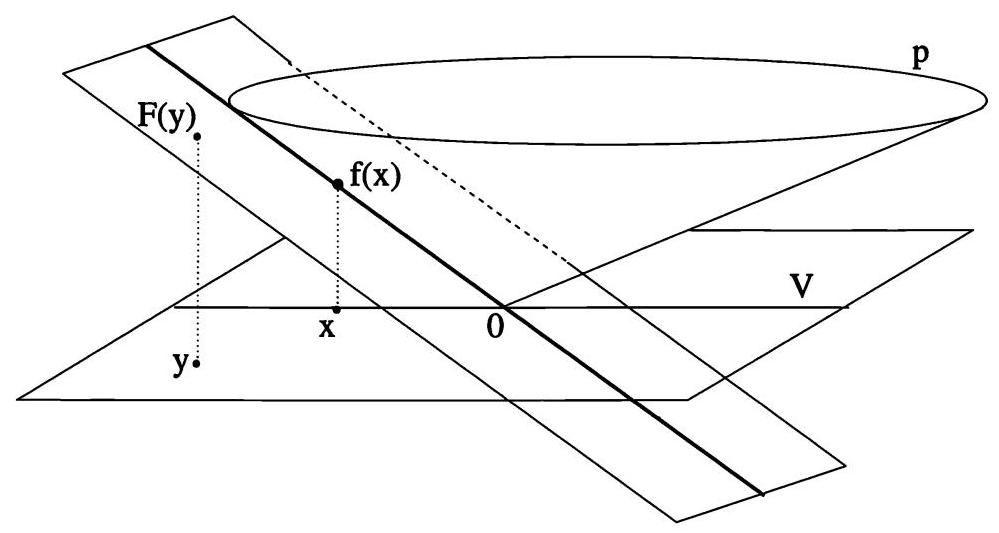
\includegraphics[width=0.9\textwidth]{images/bo_d6ik6nn7aajc739ct1l0_41_242_758_999_533_0.jpg}
\end{center}
\hspace*{3em} 

图2.5.1. 由哈恩-Banach定理，定义在子空间 \(V \subset  X\) 上、且对所有 \(x \in  V\) 满足 \(f\left( x\right)  \leq  p\left( x\right)\) 的线性泛函 \(f : V \mapsto  \mathbb{R}\) ，可延拓为一个线性泛函 \(F : X \mapsto  \mathbb{R}\) ，使得对所有 \(y \in  X\) 均有 \(F\left( y\right)  \leq  p\left( y\right)\) .

前述定理在 \(p\left( x\right)  = \; \| x\|\) 为范数的情形下具有自然应用.

定理2.30(有界线性泛函的延拓定理):设 \(X\) 为实数域或复数域 \(\mathbb{K}\) 上的赋范空间， \(f : V \mapsto  \mathbb{K}\) 为定义在子空间 \(V \subseteq  X\) 上的有界线性泛函，则 \(f\) 可延拓为一个有界线性泛函 \(F : X \mapsto  \mathbb{K}\) ，且保持范数不变:

\[
\| F\|  \doteq  \mathop{\sup }\limits_{{x \in  X,\| x\|  \leq  1}}\left| {F\left( x\right) }\right|  = \mathop{\sup }\limits_{{x \in  V,\| x\|  \leq  1}}\left| {f\left( x\right) }\right|  \doteq  \| f\| .
\]

证明:1. 首先假设 \(\mathbb{K} = \mathbb{R}\) ，即 \(f\) 取实值.令 \(\kappa  \doteq  \| f\|\) ，并定义 \(p\left( x\right)  \doteq  \kappa \| x\|\) .此时结论直接由前述定理得出.

2. 其次考虑 \(\mathbb{K} = \mathbb{C}\) 为复数域的情形.注意此时 \(V\) 与 \(X\) 亦可视为实数域上的向量空间.泛函 \(F : X \mapsto  \mathbb{C}\) 将通过分别构造其实部与虚部而得到.

对于 \(x \in  V\) ，定义 \(u\left( x\right)  \doteq  \operatorname{Re}f\left( x\right)\) .这是 \(V\) 上的一个实值线性泛函，其范数为 \(\| u\|  \leq  \kappa  \doteq  \| f\|\) .因此，由前述步骤可知，它存在一个延拓 \(U : X \mapsto  \mathbb{R}\) ，且范数为 \(\| U\|  \leq  \kappa\) .我们声称该映射

\[
F\left( x\right)  \doteq  U\left( x\right)  - {iU}\left( {ix}\right)
\]

满足全部要求.事实上，对任意 \(x \in  V\) ，

\[
F\left( x\right)  = \operatorname{Re}f\left( x\right)  - i\operatorname{Re}f\left( {ix}\right)  = \operatorname{Re}f\left( x\right)  + i\operatorname{Im}f\left( x\right)  = f\left( x\right) .
\]

此外，设 \(\alpha  \in  \mathbb{C}\) 满足 \(\left| \alpha \right|  = 1,{\alpha F}\left( x\right)  = \left| {F\left( x\right) }\right|\) .则

\[
\left| {F\left( x\right) }\right|  = {\alpha F}\left( x\right)  = U\left( {\alpha x}\right)  \leq  \kappa \| {\alpha x}\|  = \kappa \| x\| .
\]

故 \(\| F\|  \leq  \kappa  \doteq  \| f\|\) .

推论 2.31.设 \(X\) 为 Banach 空间.对任意两个向量 \(x,y \in  X\) ，若 \(x \neq  y\) ，则存在连续线性泛函 \(\phi  : X \mapsto  \mathbb{K}\) ，使得 \(\phi \left( x\right)  \neq  \phi \left( y\right)\) .

推论 2.32.设 \(X\) 为 Banach 空间.对任意向量 \(x \in  X\) ，存在连续线性泛函 \(\phi  : X \mapsto  \mathbb{K}\) ，使得 \(\phi \left( x\right)  = \| x\|\) 且 \(\| \phi \|  = 1.\) .

\begin{center}
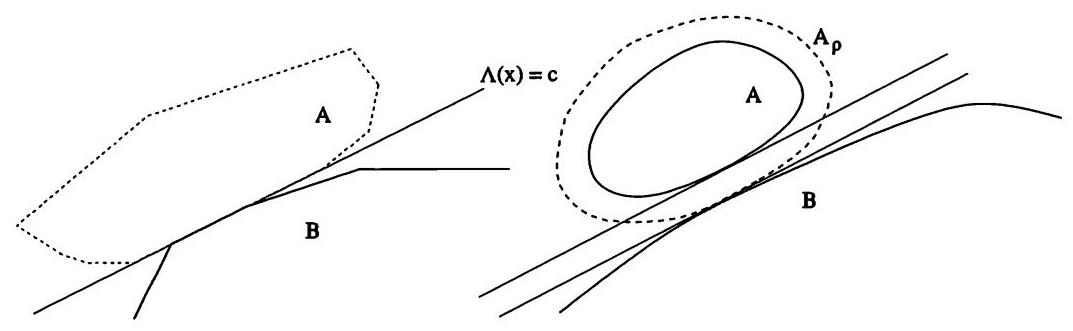
\includegraphics[width=1.0\textwidth]{images/bo_d6ik6nn7aajc739ct1l0_42_203_1420_1073_331_0.jpg}
\end{center}
\hspace*{3em} 

图 2.5.2.左:若 \(A\) 是开集，则不相交的凸集 \(A,B\) 可被一超平面分离.右:若 \(A\) 是紧集且 \(B\) 是闭集，则不相交的凸集 \(A,B\) 可被严格分离.

\section*{2.6. 凸集的分离}

考虑如下问题:给定赋范空间 \(X\) 中两个不相交的凸集 \(A,B\) ，能否找到一个有界线性泛函 \(\phi  : X \mapsto  \mathbb{R}\) ，使得像集 \(\phi \left( A\right)\) 与 \(\phi \left( B\right)\) 不相交？以下定理在 Hahn-Banach 延拓定理基础上给出了肯定回答.

定理 2.33(凸集的分离).设 \(X\) 为实数域上的赋范空间， \(A,B\) 是 \(X\) 中两个非空、不相交的凸子集.

(i) 若 \(A\) 是开集，则存在有界线性泛函 \(\phi  : X \mapsto  \mathbb{R}\) 及某数 \(\mathrm{c} \in  \mathbb{R}\) ，使得

\begin{equation}\tag{2.31}
\phi \left( a\right)  < c \leq  \phi \left( b\right) \;\text{ for all }a \in  A,b \in  B.
\end{equation}

(ii) 若 \(A\) 是紧集且 \(B\) 是闭集，则存在有界线性泛函 \(\phi  : X \mapsto  \mathbb{R}\) 及某些数 \({c}_{1},{c}_{2} \in  \mathbb{R}\) ，使得

\begin{equation}\tag{2.32}
\phi \left( a\right)  \leq  {c}_{1} < {c}_{2} \leq  \phi \left( b\right) \;\text{ for all }a \in  A,b \in  B.
\end{equation}

证明.1. 选取点 \({a}_{0} \in  A\) 与 \({b}_{0} \in  B\) ，并令 \({x}_{0} \doteq  {b}_{0} - {a}_{0}\) .考虑开集

\[
\Omega  \doteq  A - B + {x}_{0} \doteq  \left\{  {\left( {a - {a}_{0}}\right)  + \left( {{b}_{0} - b}\right) ;a \in  A,b \in  B}\right\}  .
\]

由于 \(A,B\) 是凸集且 \(A\) 是开集，显然 \(\Omega\) 是原点的一个开凸邻域.此外， \({x}_{0} \notin  \Omega\) ，否则

\[
{x}_{0} = a - b + {x}_{0},\;a - b = 0,\;\text{ for some }a \in  A,b \in  B.
\]

这与 \(A \cap  B = \varnothing\) 矛盾.

2. 考虑泛函

\begin{equation}\tag{2.33}
p\left( x\right)  \doteq  \inf \{ \lambda  \geq  0;x \in  {\lambda \Omega }\} .
\end{equation}

由于 \(\Omega\) 是原点的一个邻域，故存在某个 \(\rho  > 0\) 使得 \(B\left( {0,\rho }\right)  \subseteq  \Omega\) 成立.因此

\begin{equation}\tag{2.34}
p\left( x\right)  \leq  \frac{\| x\| }{\rho }\;\text{ for all }x \in  X.
\end{equation}

此外， \(\Omega\) 的凸性意味着(2.35)

\(p\left( {x + y}\right)  \leq  p\left( x\right)  + p\left( y\right) ,\;p\left( {tx}\right)  = {tp}\left( x\right) \;\) 对所有 \(x,y \in  X,t \geq  0.\) 成立

注意 \(p\left( {x}_{0}\right)  \geq  1\) ，因为 \({x}_{0} \notin  \Omega\) .

3. 在一维子空间 \(V \doteq  \left\{  {t{x}_{0};t \in  \mathbb{R}}\right\}\) 上，通过设定 \(f\left( {t{x}_{0}}\right)  \doteq  t\) 来定义线性泛函 \(f\) .观察可知

\[
f\left( {x}_{0}\right)  = 1,\;f\left( {t{x}_{0}}\right)  = t \leq  {tp}\left( {x}_{0}\right)  \leq  p\left( {t{x}_{0}}\right) .
\]

由哈恩-Banach延拓定理，存在一个线性泛函 \(\phi  : X \mapsto  \mathbb{R}\) ，使得

\[
- p\left( {-x}\right)  \leq  \phi \left( x\right)  \leq  p\left( x\right) \;\text{ for all }x \in  X.
\]

由(2.34)式显然可知 \(\phi\) 有界.事实上， \(\| \phi \|  \leq  {\rho }^{-1}\) .

4. 若此时 \(a \in  A\) 且 \(b \in  B\) ，则有

\[
\phi \left( a\right)  - \phi \left( b\right)  + 1 = \phi \left( {a - b + {x}_{0}}\right)  \leq  p\left( {a - b + {x}_{0}}\right)  < 1
\]

因为 \(\phi \left( {x}_{0}\right)  = f\left( {x}_{0}\right)  = 1\) ，而 \(a - b + {x}_{0} \in  \Omega\) 且 \(\Omega\) 是开集.因此

\[
\phi \left( a\right)  < \phi \left( b\right) \;\text{ for all }a \in  A,b \in  B.
\]

\(\phi \left( A\right)\) 与 \(\phi \left( B\right)\) 是 \(\mathbb{R}\) 中两个非空、不相交的凸集，且 \(\phi \left( A\right)\) 为开集.取 \(c \doteq  \mathop{\sup }\limits_{{a \in  A}}\phi \left( a\right)\) ，则结论(2.31)成立.这证明了(i).

5. 为证明(ii)，注意到关于 \(A,B\) 的假设意味着

\[
d\left( {A,B}\right)  \doteq  \inf \{ \| a - b\| ;a \in  A,b \in  B\}  > 0.
\]

若选取 \(\rho  \doteq  d\left( {A,B}\right)\) ，则以 \(A\) 为中心、半径为 \(\rho\) 的开邻域 \({A}_{\rho } \doteq  \{ x \in \; X;d\left( {x,A}\right)  < \rho \}\) 不与 \(B\) 相交.因此可将(i)应用于不相交凸集 \({A}_{\rho }\) 与 \(B\) ，从而得到一个连续线性泛函 \(\phi  : X \mapsto  \mathbb{R}\) 及一个常数 \({c}_{2}\) ，使得

\[
\phi \left( x\right)  < {c}_{2} \leq  \phi \left( y\right) \;\text{ for all }x \in  {A}_{\rho },y \in  B.
\]

我们进一步注意到，集合 \(\phi \left( A\right)\) 是紧的，因其为连续映射下紧集的像.故 \({c}_{1} \doteq  \mathop{\sup }\limits_{{x \in  A}}\phi \left( x\right)  < {c}_{2}\) .这完成了(ii)的证明.

\begin{center}
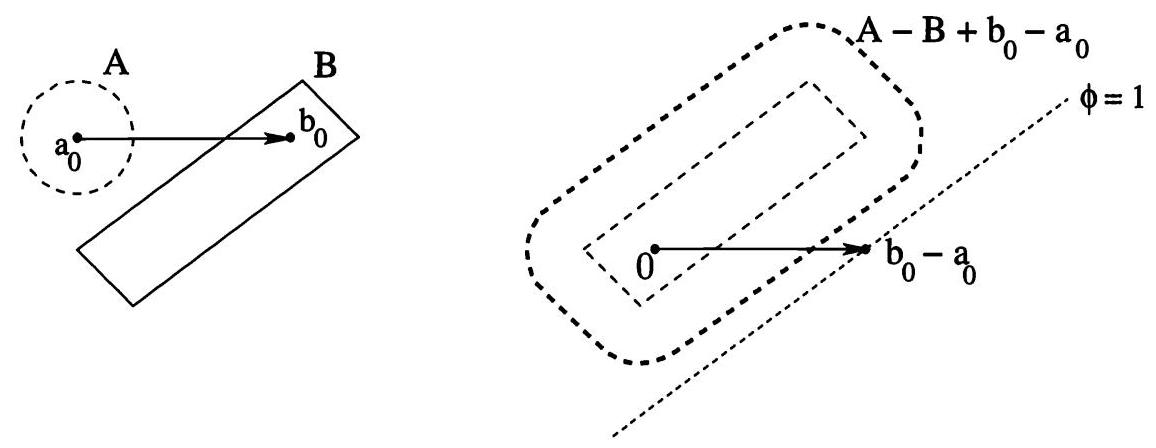
\includegraphics[width=1.0\textwidth]{images/bo_d6ik6nn7aajc739ct1l0_44_155_1289_1156_448_0.jpg}
\end{center}
\hspace*{3em} 

图2.6.1. 分离定理证明中所用的构造.

\section*{2.7. 对偶空间与弱收敛}

设 \(X\) 为实数域或复数域 \(\mathbb{K}\) 上的Banach空间.所有连续线性泛函 \(\varphi  : X \mapsto  \mathbb{K}\) 构成的集合称为 \(X\) 的对偶空间，记作 \({X}^{ * }\) .

注意，线性泛函 \(\varphi  : X \mapsto  \mathbb{K}\) 可视为一种线性算子 \(\varphi  : X \mapsto  Y\) ，特例为 \(Y = \mathbb{K}\) 时.因此我们可以使用

定理2.12，并得出 \({X}^{ * } = \mathcal{B}\left( {X,\mathbb{K}}\right)\) 是一个赋范空间，其范数为

\begin{equation}\tag{2.36}
\| \varphi {\| }_{ * } \doteq  \mathop{\sup }\limits_{{\| x\|  \leq  1}}\left| {\varphi \left( x\right) }\right| .
\end{equation}

2.7.1 弱收敛.Banach空间 \(X\) 中的一列 \({x}_{1},{x}_{2},\ldots\) 称为弱收敛的，若存在 \(x \in  X\) 使得

\[
\mathop{\lim }\limits_{{n \rightarrow  \infty }}\varphi \left( {x}_{n}\right)  = \varphi \left( x\right) \;\text{ for all }\varphi  \in  {X}^{ * }.
\]

此时，称 \(x\) 为序列 \({x}_{n}\) 的弱极限，并记作 \({x}_{n} \rightharpoonup  x\) .我们回顾:序列 \({x}_{n}\) 强收敛于 \(x\) 当且仅当 \(\begin{Vmatrix}{{x}_{n} - x}\end{Vmatrix} \rightarrow\) →0.由于按定义每个 \(\varphi  \in  {X}^{ * }\) 都是连续的，故强收敛 \({x}_{n} \rightarrow  x\) 显然蕴含弱收敛 \({x}_{n} \rightharpoonup  x\) .

若弱极限存在，则必唯一: \({x}_{n} \rightharpoonup  x\) 与 \({x}_{n} \rightharpoonup  y\) 蕴含 \(x = y\) .事实上，假设 \(y \neq  x\) .则由推论2.31，存在连续线性泛函 \(\phi  \in  {X}^{ * }\) 使得 \(\phi \left( x\right)  \neq  \phi \left( y\right)\) .这导致矛盾，因为

\[
\phi \left( x\right)  = \mathop{\lim }\limits_{{n \rightarrow  \infty }}\phi \left( {x}_{n}\right)  = \phi \left( y\right) .
\]

2.7.2 弱*收敛.可换一视角观察:每个向量 \(x \in  X\) 在 \({X}^{ * }\) 上确定一个线性泛函，即

\begin{equation}\tag{2.37}
\varphi  \mapsto  \varphi \left( x\right) ,\;\varphi  \in  {X}^{ * }.
\end{equation}

由推论2.32，该泛函的范数为

\begin{equation}\tag{2.38}
\| x{\| }_{* * } \doteq  \mathop{\sup }\limits_{{\| \varphi {\| }_{ * } \leq  1}}\left| {\varphi \left( x\right) }\right|  = \| x\| .
\end{equation}

于是我们得到标准嵌入 \(\iota  : X \mapsto  {\left( {X}^{ * }\right) }^{ * }\) :对每个元素 \(x \in  X\) ，对应一个定义在对偶空间 \({X}^{ * }\) 上的有界线性泛函 \(\iota \left( x\right)\) ，即映射 \(\varphi  \mapsto  \varphi \left( x\right)\) .由(2.38)可知，该嵌入是等距的，即保持范数.

若 \({X}^{ * }\) 上每个有界线性泛函均可表为(2.37)的形式(对某个 \(x \in  X\) )，则 \(\iota \left( X\right)  = {\left( {X}^{ * }\right) }^{ * }\) ，此时称空间 \(X\) 是自反的.自反空间的例子包括所有有限维空间，以及例2.5与例2.6中的空间 \({\mathbf{L}}^{p}\left( \Omega \right) ,{\ell }^{p}\) ，其中 \(1 < p < \infty\) .

须注意，一般情况下，空间 \({\left( {X}^{ * }\right) }^{ * }\) 可能严格大于 \(\iota \left( X\right)\) .非自反空间的例子包括空间 \({\mathbf{L}}^{1}\left( \Omega \right) ,{\mathbf{L}}^{\infty }\left( \Omega \right) ,{\ell }^{1}\) 与 \({\ell }^{\infty }\) .

嵌入 \(\iota  : X \mapsto  {\left( {X}^{ * }\right) }^{ * }\) 可用于在对偶空间 \({X}^{ * }\) 上引入弱*拓扑.我们称一列有界线性泛函 \({\varphi }_{n} \in  {X}^{ * }\) 弱*收敛于 \(\varphi  \in  {X}^{ * }\) ，并记作 \({\varphi }_{n} \rightarrow  \varphi\) ，若

\begin{equation}\tag{2.39}
\mathop{\lim }\limits_{{n \rightarrow  \infty }}{\varphi }_{n}\left( x\right)  = \varphi \left( x\right) \;\text{ for every }x \in  X.
\end{equation}

这比按范数收敛 \({\varphi }_{n} \rightarrow  \varphi\) 弱得多.事实上

\({\varphi }_{n}\overset{ * }{ \rightharpoonup  }\varphi \;\) 表示对每个 \(x \in  X, \; {\varphi }_{n} \rightarrow  \varphi \;\) ，有 \(\;\left| {{\varphi }_{n}\left( x\right)  - \varphi \left( x\right) }\right|  \rightarrow  0\;\) ； \(\;\mathop{\sup }\limits_{{x \in  X,\| x\|  \leq  1}}\left| {{\varphi }_{n}\left( x\right)  - \varphi \left( x\right) }\right|  \rightarrow  0.\)

由定理2.22可知，若空间 \({X}^{ * }\) 是无限维的，则闭单位球 \({B}_{1} \subset  {X}^{ * }\) 不是紧集:可找到一族线性泛函 \({\varphi }_{n} \in  {X}^{ * }\) ，满足对每个 \(n \geq  1\) 均有 \({\begin{Vmatrix}{\varphi }_{n}\end{Vmatrix}}_{ * } \leq  1\) ，但其中不存在任何(关于 \({X}^{ * }\) 的范数拓扑)收敛子列.另一方面，若将强收敛改为仅要求弱*收敛，则可得到肯定结果.

定理2.34(Banach-Alaoglu定理).设 \(X\) 为可分Banach空间.则任意有界线性泛函序列 \({\varphi }_{n} \in  {X}^{ * }\) 均存在弱*收敛子列.\footnote{Banach-Alaoglu定理即使在不假设 \(X\) 可分的情况下仍成立.对此更一般情形的证明，参见 \(\left\lbrack  {\mathbf{C},\mathbf{R}}\right\rbrack\) .}

证明.1. 考虑有界线性泛函序列 \({\varphi }_{n} \in  {X}^{ * }\) ，例如对所有 \(n \geq  1\) 均有 \({\begin{Vmatrix}{\varphi }_{n}\end{Vmatrix}}_{ * } \leq  C\) .由于 \(X\) 可分，故存在一个可数稠密子集 \(S = \left\{  {{x}_{1},{x}_{2},\ldots }\right\}   \subset  X\) .

2. 我们断言存在一个子列 \({\left( {\varphi }_{{n}_{j}}\right) }_{j \geq  1}\) ，它在每一点 \({x}_{k}\) 处点态收敛，即

\begin{equation}\tag{2.40}
\mathop{\lim }\limits_{{j \rightarrow  \infty }}{\varphi }_{{n}_{j}}\left( {x}_{k}\right)  = \varphi \left( {x}_{k}\right)
\end{equation}

对某些值 \(\varphi \left( {x}_{k}\right)\) 及所有 \(k \geq  1\) 成立.该子列将通过标准对角化方法构造.

由于数列 \({\left( {\varphi }_{n}\left( {x}_{1}\right) \right) }_{n \geq  1}\) 有界，故存在一个无穷指标集 \({I}_{1} \subset  \mathbb{N}\) ，使得子列 \({\left( {\varphi }_{n}\left( {x}_{1}\right) \right) }_{n \in  {I}_{1}}\) 收敛于某个极限 \(\varphi \left( {x}_{1}\right)\) .

类似地，数列 \({\left( {\varphi }_{n}\left( {x}_{2}\right) \right) }_{n \geq  1}\) 亦有界.因此存在一个无穷指标集 \({I}_{2} \subset  {I}_{1}\) ，使得子列 \({\left( {\varphi }_{n}\left( {x}_{2}\right) \right) }_{n \in  {I}_{2}}\) 收敛于某个极限 \(\varphi \left( {x}_{2}\right)\) .

由归纳法，对每个 \(k\) ，存在一个无限指标集 \({I}_{k} \subset  {I}_{k - 1}\) ，使得子列 \({\left( {\varphi }_{n}\left( {x}_{k}\right) \right) }_{n \in  {I}_{k}}\) 收敛于某个极限 \(\varphi \left( {x}_{k}\right)\) .

现选取子列 \({n}_{1} < {n}_{2} < {n}_{3} < \cdots\) ，满足对每个 \(j\) 均有 \({n}_{j} \in  {I}_{j}\) .由于 \(j \rightarrow  \infty\) ，由此得到对每个 \(k \geq  1\) 均有收敛性 \({\varphi }_{{n}_{j}}\left( {x}_{k}\right)  \rightarrow  \varphi \left( {x}_{k}\right)\) .

3. 我们声称极限函数 \(\varphi  : S \mapsto  \mathbb{K}\) 是Lipschitz连续的，其Lipschitz常数为 \(C = \mathop{\sup }\limits_{n}{\begin{Vmatrix}{\varphi }_{n}\end{Vmatrix}}_{ * }\) .事实上，对每个 \({x}_{h},{x}_{k} \in  S\) ，有

\[
\left| {\varphi \left( {x}_{h}\right)  - \varphi \left( {x}_{k}\right) }\right|  = \mathop{\lim }\limits_{{j \rightarrow  \infty }}\left| {{\varphi }_{{n}_{j}}\left( {x}_{h}\right)  - {\varphi }_{{n}_{j}}\left( {x}_{k}\right) }\right|
\]

\[
\leq  \mathop{\limsup }\limits_{{j \rightarrow  \infty }}{\begin{Vmatrix}{\varphi }_{{n}_{j}}\end{Vmatrix}}_{ * }\begin{Vmatrix}{{x}_{h} - {x}_{k}}\end{Vmatrix} \leq  C\begin{Vmatrix}{{x}_{h} - {x}_{k}}\end{Vmatrix}.
\]

因此，映射 \(\varphi\) 可通过连续性唯一延拓至 \(S\) 的闭包，即整个空间 \(X\) .该连续延拓仍记为 \(\varphi  : X \mapsto  \mathbb{K}\) .

4. 剩余需证子列 \({\varphi }_{{n}_{j}}\) 弱*收敛于 \(\varphi\) .任给 \(x \in  X\) 与 \(\varepsilon  > 0\) .由于 \(S\) 稠密，可选取一点 \({x}_{k} \in  S\) 使得 \(\begin{Vmatrix}{{x}_{k} - x}\end{Vmatrix} < \varepsilon\) .注意到所有函数 \({\varphi }_{n}\) 与 \(\varphi\) 均为Lipschitz连续，且Lipschitz常数均为 \(C\) ，故有

\[
\mathop{\limsup }\limits_{{j \rightarrow  \infty }}\left| {{\varphi }_{{n}_{j}}\left( x\right)  - \varphi \left( x\right) }\right|
\]

\[
\leq  \mathop{\limsup }\limits_{{j \rightarrow  \infty }}\left| {{\varphi }_{{n}_{j}}\left( x\right)  - {\varphi }_{{n}_{j}}\left( {x}_{k}\right) }\right|
\]

\[
+ \mathop{\limsup }\limits_{{j \rightarrow  \infty }}\left| {{\varphi }_{{n}_{j}}\left( {x}_{k}\right)  - \varphi \left( {x}_{k}\right) }\right|  + \left| {\varphi \left( {x}_{k}\right)  - \varphi \left( x\right) }\right|
\]

\[
\leq  C\begin{Vmatrix}{x - {x}_{k}}\end{Vmatrix} + 0 + C\begin{Vmatrix}{{x}_{k} - x}\end{Vmatrix} \leq  {2C\varepsilon }.
\]

由于 \(\varepsilon  > 0\) 是任意的，这表明当 \(j \rightarrow  \infty\) 时 \(\left| {{\varphi }_{{n}_{j}}\left( x\right)  - \varphi \left( x\right) }\right|  \rightarrow  0\) ，从而证得弱*收敛 \({\varphi }_{{n}_{j}}\overset{ * }{ \rightharpoonup  }\varphi\) .

作为一致有界线性泛函序列的逐点极限，显然映射 \(\varphi\) 本身也是有界且线性的.

\section*{2.8. 习题}

1. 判断下列集合是否为赋范空间.若否，指出哪个性质(N1)-(N3)不成立；若是，进一步判断其是否为Banach空间.

(i) 设 \(X = \mathbb{R}\) ，其中

\[
\| x\|  = \begin{cases} x & \text{ if }x \geq  0, \\   - {2x} & \text{ if }x < 0. \end{cases}
\]

(ii) 设 \(X\) 为实数列 \(x = \left( {{x}_{1},{x}_{2},{x}_{3},\ldots }\right)\) 构成的向量空间，其中除有限个 \(k\) 外均有 \({x}_{k} = 0\) .在 \(X\) 上取范数(2.8).

(iii) 设 \(X\) 为所有多项式(任意次数)构成的空间，其范数为 \(\| p\|  = \; \mathop{\max }\limits_{{x \in  \left\lbrack  {0,1}\right\rbrack  }}\left| {p\left( x\right) }\right|\) .

(iv) 设 \(X\) 为所有次数为 \(\leq  2\) 的多项式构成的空间，其范数为

\[
\| p\|  \doteq  \left| {p\left( 0\right) }\right|  + \left| {{p}^{\prime }\left( 0\right) }\right|  + \left| {{p}^{\prime \prime }\left( 0\right) }\right| .
\]

(v) 设 \(X\) 为区间 \(\left\lbrack  {0,1}\right\rbrack\) 上所有连续函数构成的空间，其中

\[
\| f\|  \doteq  {\int }_{0}^{1}\left| {f\left( x\right) }\right| {dx}
\]

(vi) 固定 \(\kappa  \in  \mathbb{R}\) ，并令 \(X\) 为所有满足以下条件的连续函数 \(f : \lbrack 0,\infty \lbrack  \mapsto  \mathbb{R}\) 构成的空间:

\[
\| f\|  \doteq  \mathop{\sup }\limits_{{t \geq  0}}{e}^{\kappa t}\left| {f\left( t\right) }\right|  < \infty .
\]

(vii) 设 \(X = {\mathbb{R}}^{2}\) .给定 \(x = \left( {{x}_{1},{x}_{2}}\right)\) ，对固定的 \(0 < p < 1\) ，定义

\[
\| x\|  \doteq  {\left( {\left| {x}_{1}\right| }^{p} + {\left| {x}_{2}\right| }^{p}\right) }^{1/p}.
\]

注:关于 (vii)，值得检验的是

\[
d\left( {x,y}\right)  \doteq  {\left| {x}_{1} - {y}_{1}\right| }^{1/2} + {\left| {x}_{2} - {y}_{2}\right| }^{1/2}
\]

是否为 \({\mathbb{R}}^{2}\) 上的一个距离.开球 \(B\left( {x,r}\right)  = \{ y;d\left( {y,x}\right)  < r\}\) 是否为凸集？ \(d\left( {\cdot , \cdot  }\right)\) 是否平移不变？

2. 设 \(X,Y\) 为 Banach 空间.证明其笛卡尔积

\[
X \times  Y = \{ \left( {x,y}\right) ;x \in  X,y \in  Y\}
\]

在范数

\begin{equation}\tag{2.41}
\| \left( {x,y}\right) \|  \doteq  \max \{ \| x\| ,\| y\| \} .
\end{equation}

3. 设 \(X\) 为实数域或复数域 \(\mathbb{K}\) 上的 Banach 空间.注意: \(X \times  X\) 和 \(\mathbb{K} \times  X\) 均为 Banach 空间，其乘积范数如 (2.41) 所示.证明:

(i) 映射 \(\left( {x,y}\right)  \mapsto  x + y\) 从 \(X \times  X\) 到 \(X\) 是连续的.

(ii) 映射 \(\left( {\alpha ,x}\right)  \mapsto  {\alpha x}\) 从 \(\mathbb{K} \times  X\) 到 \(X\) 是连续的.

4. 设 \(X\) 为具有范数 \(\|  \cdot  \|\) 的赋范空间.证明:任一子空间 \(V \subset  X\) 在同一范数下也构成赋范空间.若 \(X\) 是 Banach 空间且 \(V\) 是闭的，则 \(V\) 也是 Banach 空间.

5. 证明:赋范空间 \(X\) 完备当且仅当每个绝对收敛级数均有和:

\[
\mathop{\sum }\limits_{{k \geq  1}}\begin{Vmatrix}{x}_{k}\end{Vmatrix} < \infty \;\text{ implies that }\;\mathop{\sum }\limits_{{k \geq  1}}{x}_{k} \doteq  \mathop{\lim }\limits_{{n \rightarrow  \infty }}\mathop{\sum }\limits_{{k = 1}}^{n}{x}_{k}\;\text{ exists. }
\]

6. 设 \(X\) 为向量空间.集合 \(A \subset  X\) 的凸包定义为 \(A\) 中元素的所有凸组合构成的集合，即

\[
\operatorname{co}A \doteq  \left\{  {\mathop{\sum }\limits_{{k = 1}}^{N}{\theta }_{k}{a}_{k};N \geq  1,{a}_{k} \in  A,{\theta }_{k} \in  \left\lbrack  {0,1}\right\rbrack  ,\mathop{\sum }\limits_{{k = 1}}^{N}{\theta }_{k} = 1}\right\}  .
\]

证明:(i) \(\operatorname{co}A\) 是凸集；(ii) \(\operatorname{co}A\) 是所有包含 \(A\) 的凸集的交集.

7. 设 \(X\) 为 Banach 空间，且 \(A,B \subset  X\) .证明下列命题.

(i) 若 \(A\) 是开集，则 \(\operatorname{co}A\) 也是开集.

(ii) 若 \(A\) 是有界集，则 co \(A\) 也是有界集.

(iii) 若 \(A,B\) 是有界集，则集合 \(A + B \doteq  \{ a + b;a \in  A,b \in  B\}\) 也是有界集.

(iv) 若 \(A\) 是闭集且 \(B\) 是紧集，则 \(A + B\) 是闭集.

(v) 两个闭集的和未必是闭集.

(vi) 若 \(A\) 是凸集，则 \(A + A \doteq  \{ x + y;x \in  A,y \in  A\}  = {2A} \doteq  \{ {2x};x \in  A\}\) .

(vii) 若 \(A\) 是闭集且 \(A + A = {2A}\) ，则 \(A\) 必为凸集.

8. 设 \(X\) 是赋范空间.若集合 \(S \subseteq  X\) 满足 \(a \in  S\) 蕴含 \(- a \in  S\) ，则称其为对称集.证明:

(i) 若 \(S\) 是凸集，则其闭包也是凸集.

(ii) 若 \(S\) 是对称集，则其闭包也是对称集.

9. 设 \(X,Y\) 是实数域上的Banach空间， \(\Lambda  : X \mapsto  Y\) 是有界线性算子.证明:

(i) 若 \(S\) 是凸集，则其像 \(\Lambda \left( S\right)\) 是凸集.

(ii) 若 \(S\) 是对称集，则其像 \(\Lambda \left( S\right)\) 是对称集.

10. 设 \(\Lambda  : X \mapsto  Y\) 是线性算子.假设对任一序列 \({x}_{n} \rightarrow  0\) ，序列 \({\left( \Lambda {x}_{n}\right) }_{n \geq  1}\) 均有界.证明: \(\Lambda\) 是连续的.

11. 设 \(X\) 是无限维Banach空间， \(S\) 是一组线性无关向量.记 span \(\left( S\right)\) 为 \(S\) 中元素的所有(有限)线性组合构成的集合.证明:

(i) 若 \(S = \left\{  {{v}_{1},\ldots ,{v}_{N}}\right\}\) 是有限集，则 \(\operatorname{span}\left( S\right)\) 是 \(X\) 的闭子空间.

(ii) 若 \(S = \left\{  {{v}_{k};k \geq  1}\right\}\) 为无穷序列，则向量空间span \(\left( S\right)\) 在 \(X\) 中不可能是闭的.

12(实数域与复数域上的空间).设 \(X\) 为复数域上的向量空间，则 \(X\) 亦为实数域上的向量空间.若 \(\Phi  : X \mapsto  \mathbb{C}\) 为复线性泛函， \(\phi \left( x\right)  = \operatorname{Re}\Phi \left( x\right)\) 为其实部，证明 \(\phi\) 为实线性泛函，且 \(\Phi \left( x\right)\) 可由 \(\phi\) 按如下方式重构:

\[
\Phi \left( x\right)  = \phi \left( x\right)  - {i\phi }\left( {ix}\right) .
\]

13. 证明赋范空间 \(X\) 是有限维的当且仅当其对偶空间 \({X}^{ * }\) 是有限维的.

14. 考虑例2.6与2.7中定义的实数序列空间 \({\ell }^{p}\) .若 \(1 \leq  p \leq  q \leq  \infty\) ，则 \({\ell }^{p} \subseteq  {\ell }^{q}\) ，且等号成立当且仅当 \(p = q\) .此外，证明恒等算子 \(\Lambda  : {\ell }^{p} \mapsto  {\ell }^{q}\) (定义为 \(\Lambda \mathbf{x} = \mathbf{x}\) )对每个 \(p \leq  q\) 均连续.

15. 对 \(1 \leq  p < \infty\) ，证明(2.10)中引入的子空间 \(V \doteq  \operatorname{span}\left\{  {{\mathbf{e}}_{k};k \geq  1}\right\}\) 在空间 \({\ell }^{p}\) 中稠密.对 \(p = \infty\) ，证明 \(V\) 的闭包恰为所有收敛于零的序列构成的子空间 \({c}_{0}\) .

16.(对角算子的性质)对 \(1 \leq  p \leq  \infty\) ，考虑(2.13)中定义的算子 \(\Lambda  : {\ell }^{p} \mapsto  {\ell }^{p}\) .证明例2.14中(i)-(ii)项断言.

17. 补全例2.18的细节:即固定 \(1 \leq  p \leq  \infty\) ，并设 \(g : \Omega  \mapsto  \mathbb{R}\) 为任意可测函数.

(i) 若 \(g \in  {\mathbf{L}}^{\infty }\left( \Omega \right)\) ，证明乘法算子 \({M}_{g} : f \mapsto  {gf}\) 从 \({\mathbf{L}}^{p}\left( \Omega \right)\) 到自身的映射是有界的，且其范数由(2.15)给出.

(ii) 若 \(g \notin  {\mathbf{L}}^{\infty }\left( \Omega \right)\) ，证明线性算子 \(f \mapsto  {gf}\) 从 \({\mathbf{L}}^{p}\left( \Omega \right)\) 到自身的映射是无界的.直接证明 \(\operatorname{Dom}\left( {M}_{g}\right)  \neq  {\mathbf{L}}^{p}\left( \Omega \right)\) .

18. 固定 \(1 \leq  p \leq  \infty\) .设 \({\left( {f}_{n}\right) }_{n \geq  1}\) 为 \({\mathbf{L}}^{p}\left( \mathbb{R}\right)\) 中一列弱收敛于函数 \(f \in  {\mathbf{L}}^{p}\left( \mathbb{R}\right)\) 的函数.证明:

\[
\mathop{\lim }\limits_{{n \rightarrow  \infty }}{\int }_{a}^{b}{f}_{n}\left( x\right) {dx} = {\int }_{a}^{b}f\left( x\right) {dx}\;\text{ for all }a < b.
\]

19. 考虑下列函数序列

\[
{f}_{n}\left( x\right)  = \left\{  \begin{matrix} 1/n & & \text{ if }x \in  \left\lbrack  {0,n}\right\rbrack  , \\  0 & & \text{ otherwise. } \end{matrix}\right.
\]

(i) 证明: \({f}_{n} \rightarrow  0\) 在每个满足 \(1 < p \leq  \infty\) 的空间 \({\mathbf{L}}^{p}\left( \mathbb{R}\right)\) 中强收敛(即 \(\begin{Vmatrix}{f}_{n}\end{Vmatrix} \rightarrow  0\) ).

(ii) 另一方面，证明:在空间 \({\mathbf{L}}^{1}\left( \mathbb{R}\right)\) 中，该序列不强收敛；事实上，该序列甚至不存在任何弱收敛子列.

20. 设 \(Y\) 是 Banach 空间 \(X\) 的子空间， \(\Lambda  : Y \mapsto  {\mathbb{R}}^{n}\) 是从 \(Y\) 到欧氏空间 \({\mathbb{R}}^{n}\) 的有界线性算子.证明: \(\Lambda\) 可延拓为一线性算子 \(\widetilde{\Lambda } : X \mapsto  {\mathbb{R}}^{n}\) ，其范数为 \(\| \widetilde{\Lambda }\|  \leq  \sqrt{n}\| \Lambda \|\) .

21. 设 \(\phi  : {\mathbb{R}}^{2} \mapsto  \mathbb{R}\) 是一线性泛函，记为 \(\phi \left( {{x}_{1},{x}_{2}}\right)  = a{x}_{1} + b{x}_{2}\) .给出如下结论的直接证明:

(i) 若 \({\mathbb{R}}^{2}\) 赋以范数 \(\| x{\| }_{1} = \left| {x}_{1}\right|  + \left| {x}_{2}\right|\) ，则相应算子范数(2.36)为 \(\| \phi {\| }_{\infty } = \max \{ \left| a\right| ,\left| b\right| \}\) .

(ii) 若 \({\mathbb{R}}^{2}\) 赋以范数 \(\| x{\| }_{\infty } = \max \left\{  {\left| {x}_{1}\right| ,\left| {x}_{2}\right| }\right\}\) ，则相应范数(2.36)为 \(\| \phi {\| }_{1} = \left| a\right|  + \left| b\right|\) .

(iii) 若 \({\mathbb{R}}^{2}\) 赋以范数 \(\| x{\| }_{p} = {\left( {\left| {x}_{1}\right| }^{p} + {\left| {x}_{2}\right| }^{p}\right) }^{1/p}\) ，其中 \(1 < p < \; \infty\) ，则相应范数(2.36)为 \(\| \phi {\| }_{q} = {\left( {\left| a\right| }^{q} + {\left| b\right| }^{q}\right) }^{1/q}\) ，其中 \(\frac{1}{p} + \frac{1}{q} = 1\)

22. 设 \(X\) 是一矢量空间， \(B \subset  X\) 是其凸子集，且对任一非零向量 \(x \in  X\) ，均存在正数 \({\theta }_{x} > 0\) ，使得

\({\alpha x} \in  B\) 当且仅当 \(\left| \alpha \right|  \leq  {\theta }_{x}.\)

对 \(r \geq  0\) ，记 \({rB} \doteq  \{ {rb};b \in  B\}\) .证明:

\[
\| x\|  \doteq  \min \{ r \geq  0;x \in  {rB}\}
\]

是 \(X\) 上的一个范数，且 \(B = \{ x \in  X;\| x\|  \leq  1\}\) 是该范数下的单位球.

23. 设 \(\Omega  \subseteq  {\mathbb{R}}^{n}\) 为开集.在(可能无界)连续函数 \(f : \Omega  \mapsto  \mathbb{R}\) 的空间 \(\mathcal{C}\left( \Omega \right)\) 上，考虑半范数 \({p}_{k}\left( \cdot \right)\) 和在 (2.22)、(2.20) 中定义的距离 \(d\left( {\cdot , \cdot  }\right)\) .

接下来，考虑任意一列开集 \({A}_{k}^{\prime }\) ，其紧致地包含于 \(\Omega\) 中，且满足 \(\mathop{\bigcup }\limits_{{k > 1}}{A}_{k}^{\prime } = \Omega\) .如前定义半范数 \({p}_{k}^{\prime }\left( \cdot \right)\) 与距离 \({d}^{\prime }\left( {\cdot , \cdot  }\right)\) ，但将(2.21)中的集合 \({A}_{k}\) 替换为集合 \({A}_{k}^{\prime }\) .

证明两个距离 \(d,{d}^{\prime }\) 等价.即:对任意连续函数序列 \({\left( {f}_{j}\right) }_{j \geq  1}\) ，下列命题等价:

(i) 该序列关于距离 \(d\) 是Cauchy列，

(ii) 该序列关于距离 \({d}^{\prime }\) 是Cauchy列，

(iii) 函数 \({f}_{j}\) 在 \(\Omega\) 的每个紧子集上一致收敛.

24. 在空间 \(\mathcal{C}\left( \Omega \right)\) 上，考虑由(2.22)定义的半范数 \({p}_{k}\left( \cdot \right)\) 及由(2.20)构造的距离 \(d\left( {\cdot , \cdot  }\right)\) .

(i) 解释为何 \(\| f\|  \doteq  \mathop{\sum }\limits_{{k = 1}}^{\infty }{2}^{-k}{p}_{k}\left( f\right)\) 不能在 \(\mathcal{C}\left( \Omega \right)\) 上诱导出一个范数.

(ii) 考虑以0(即恒零函数)为中心的开单位球 \(B \doteq  \{ f \in  \mathcal{C}\left( \Omega \right) ;d\left( {f,0}\right)  < 1\}\) .解释为何

\[
\| f{\| }_{\diamond } \doteq  \inf \left\{  {\lambda  > 0;{\lambda }^{-1}f \in  B}\right\}
\]

不能在 \(\mathcal{C}\left( \Omega \right)\) 上诱导出一个范数.

25. 设 \(X\) 为Banach空间.考虑任意集合 \(S \subset  X\) ，并假设 \(x \in  \operatorname{span}\left( S\right)\) .证明存在点 \({x}_{j} \in  S\) 与系数 \({c}_{j} \in  \mathbb{K},j = 1,\ldots ,N\) ，使得

\begin{equation}\tag{2.42}
x = \mathop{\sum }\limits_{{j = 1}}^{N}{c}_{j}{x}_{j},\;\begin{Vmatrix}{\mathop{\sum }\limits_{{j = 1}}^{k}{c}_{j}{x}_{j}}\end{Vmatrix} \leq  2\| x\| \;\text{ for all }k = 1,\ldots ,N.
\end{equation}

26. 设 \(S\) 为Banach空间 \(X\) 的一个子集.证明下列命题等价:

(i) \(x \in  \overline{\operatorname{span}\left( S\right) }\) .

(ii) \(x = \mathop{\sum }\limits_{{j = 1}}^{\infty }{c}_{j}{x}_{j} \doteq  \mathop{\lim }\limits_{{n \rightarrow  \infty }}\mathop{\sum }\limits_{{j = 1}}^{n}{c}_{j}{x}_{j}\) ，其中点 \({x}_{j} \in  S\) 与数 \({c}_{j} \in  \mathbb{K}\) 满足某条件

27. 考虑Banach空间 \({\ell }^{\infty }\) ，其由所有实数有界序列 \(x = \; \left( {{x}_{1},{x}_{2},{x}_{3},\ldots }\right)\) 构成.

(i) 证明存在有界线性泛函 \(F : {\ell }^{\infty } \mapsto  \mathbb{R}\) ，使得

\begin{equation}\tag{2.43}
\left| {F\left( x\right) }\right|  \leq  \| x{\| }_{{\ell }^{\infty }} \doteq  \mathop{\sup }\limits_{{n \geq  1}}\left| {x}_{n}\right|
\end{equation}

\begin{equation}\tag{2.44}
F\left( x\right)  = \mathop{\lim }\limits_{{n \rightarrow  \infty }}{x}_{n}\;\text{ if the limit exists. }
\end{equation}

(ii) 证明:若 \(F : {\ell }^{\infty } \mapsto  \mathbb{R}\) 满足上述性质(2.43)-(2.44)，则

\[
\mathop{\liminf }\limits_{{n \rightarrow  \infty }}{x}_{n} \leq  F\left( x\right)  \leq  \mathop{\limsup }\limits_{{n \rightarrow  \infty }}{x}_{n}\;\text{ for all }x \in  {\ell }^{\infty }.
\]

(iii) 利用(ii)证明:若存在整数 \(N\) ，使得对所有 \(n \geq  N\) 均有 \({x}_{n} \leq  {y}_{n}\) ，则 \(F\left( x\right)  \leq  F\left( y\right)\) .

(iv) 证明:对任意序列 \(a = \left( {{a}_{1},{a}_{2},\ldots }\right)  \in  {\ell }^{1}\) ，该连续线性泛函

\[
{F}_{a}\left( x\right)  \doteq  \mathop{\sum }\limits_{{n \geq  1}}{a}_{n}{x}_{n}
\]

不可能满足(2.44).因此， \({\ell }^{\infty }\) 上所有连续线性泛函构成的空间无法与 \({\ell }^{1}\) 等同.

(v) 对每个有界实数列 \(x = \left( {{x}_{1},{x}_{2},\ldots }\right)\) ，定义

\[
\widetilde{F}\left( x\right)  \doteq  \frac{1}{2}\left( {\mathop{\liminf }\limits_{{n \rightarrow  \infty }}{x}_{n}}\right)  + \frac{1}{2}\left( {\mathop{\limsup }\limits_{{n \rightarrow  \infty }}{x}_{n}}\right) .
\]

\(\widetilde{F}\) 是否满足(2.43)-(2.44)？ \(\widetilde{F}\) 是否为Banach空间 \({\ell }^{\infty }\) 上的有界线性泛函？

28. 在Banach空间 \(X = {\mathbf{L}}^{\infty }\left( \mathbb{R}\right)\) 中，考虑由所有有界连续函数构成的子空间 \(V\) .

证明:存在一个满足 \(\| \Lambda \|  = 1\) 的有界线性泛函 \(\Lambda  : {\mathbf{L}}^{\infty }\left( \mathbb{R}\right)  \mapsto  \mathbb{R}\) ，使得对每个有界连续函数 \(f\) 均有 \({\Lambda f} \doteq  f\left( 0\right)\) .但需指出:不存在函数 \(g \in  {\mathbf{L}}^{1}\left( \mathbb{R}\right)\) ，使得对每个 \(f \in  {\mathbf{L}}^{\infty }\left( \mathbb{R}\right)\) 均有 \({\Lambda f} = \int {fgdx}\) .

由此得出: \({\mathbf{L}}^{\infty }\left( \mathbb{R}\right)\) 的对偶空间无法与 \({\mathbf{L}}^{1}\left( \mathbb{R}\right)\) 等同.

29. 设 \(X\) 为赋范空间， \(\Omega  \subset  X\) 为包含原点的开凸集.考虑泛函

\begin{equation}\tag{2.45}
p\left( x\right)  \doteq  \inf \{ \lambda  \geq  0;x \in  {\lambda \Omega }\} .
\end{equation}

(i) 证明 \(p\left( \cdot \right)\) 满足下列条件

\[
p\left( {x + y}\right)  \leq  p\left( x\right)  + p\left( y\right) ,\;p\left( {tx}\right)  = {tp}\left( x\right) \text{ for all }x,y \in  X,t \geq  0.
\]

(ii) 在假设 \({B}_{r} \doteq  \{ x \in  X;\| x\|  < r\}  \subseteq  \Omega\) 成立的前提下，证明 \(p\left( x\right)  \leq  \| x\| /r\) .

(iii) 在假设 \(\Omega  = \{ x \in  X;\| x\|  < 1\}\) 为开单位球的前提下，证明 \(p\left( x\right)  = \| x\| .\)

30. 设 \({\mathcal{C}}^{0}\left( \left\lbrack  {0,1}\right\rbrack  \right)\) 为定义在 \(\left\lbrack  {0,1}\right\rbrack   \mapsto  \mathbb{R}\) 上的所有实值连续函数 \(f\) 构成的Banach空间，其范数为 \(\| f\|  = \mathop{\max }\limits_{{x \in  \left\lbrack  {0,1}\right\rbrack  }}\left| {f\left( x\right) }\right|\) .

(i) 证明 \(X = \left\{  {f \in  {\mathcal{C}}^{0}\left( \left\lbrack  {0,1}\right\rbrack  \right) ;f\left( 0\right)  = 0}\right\}\) 是 \({\mathcal{C}}^{0}\) 的闭子空间，从而本身亦为Banach空间.

(ii) 证明映射 \(f \mapsto  {\Lambda f} \doteq  {\int }_{0}^{1}f\left( x\right) {dx}\) 是 \(X\) 上的连续线性泛函.计算其范数 \(\| \Lambda \|  \doteq  \mathop{\sup }\limits_{{\| f\|  \leq  1}}\left| {\Lambda f}\right|\) .该上确界是否在闭单位球上实际取到(即是否为最大值)？

31. 设 \(X\) 为实数域上的Banach空间， \({X}^{ * }\) 为其对偶空间.设 \(\Omega  \subset  X\) 为包含原点的凸集.定义

\[
{\Omega }^{ * } \doteq  \left\{  {\phi  \in  {X}^{ * };\phi \left( x\right)  \leq  1\text{ for all }x \in  \Omega }\right\}  ,
\]

\[
{\Omega }^{* * } \doteq  \left\{  {x \in  X;\phi \left( x\right)  \leq  1\text{ for all }\phi  \in  {\Omega }^{ * }}\right\}
\]

证明 \({\Omega }^{* * }\) 是 \(\Omega\) 的闭包.

32. 设 \(\xi\) 为实数域上Banach空间 \(X\) 中的一个非零向量.称 \(U = \; \operatorname{span}\{ \xi \}  = \{ {t\xi };t \in  \mathbb{R}\}\)

证明存在一个闭子空间 \(V \subset  X\) ，使得 \(X = U \oplus  V\) .即，每个元素 \(x \in  X\) 均可唯一地表示为如下和:

\[
x = u + v\;\text{ with }\;u \in  U,v \in  V.
\]

此外，投影算子 \(x \mapsto  u = {\pi }_{U}x\) 和 \(x \mapsto  v = {\pi }_{V}x\) 均为连续线性算子.

33. 在Banach空间 \(X = {\mathbf{L}}^{1}\left( \left\lbrack  {-1,1}\right\rbrack  \right)\) 上，证明存在一个范数为 \(\| \varphi \|  = 1\) 的连续线性泛函 \(\varphi  : X \mapsto  \mathbb{R}\) ，具有如下性质:

\[
\text{ If }f\text{ is a polynomial of degree 1, then }\varphi \left( f\right)  = {f}^{\prime }\left( 0\right) \text{ . }
\]

34. 给定开集 \(\Omega  \subset  {\mathbb{R}}^{n}\) ，记 \({\mathcal{C}}^{m}\left( \Omega \right)\) 为所有具有直至 \(m\) 阶连续偏导数的连续函数 \(f : \Omega  \mapsto  \mathbb{R}\) 构成的空间.设 \({A}_{k}\) 为 (2.21) 中定义的集合.证明半范数序列

\begin{equation}\tag{2.46}
{p}_{k}\left( f\right)  \doteq  \mathop{\sum }\limits_{{\left| \alpha \right|  \leq  m}}\mathop{\max }\limits_{{x \in  {A}_{k}}}\left| {{D}^{\alpha }f\left( x\right) }\right|
\end{equation}

使 \({\mathcal{C}}^{m}\left( \Omega \right)\) 成为Fréchet空间.此处 \(\alpha  = \left( {{\alpha }_{1},\ldots ,{\alpha }_{n}}\right)\) 是长度为 \(\left| \alpha \right|  \doteq  {\alpha }_{1} + \cdots  + {\alpha }_{n}\) 的多重指标，且 \({D}^{\alpha }f \doteq  {\left( \frac{\partial }{\partial {x}_{1}}\right) }^{{\alpha }_{1}}\cdots {\left( \frac{\partial }{\partial {x}_{n}}\right) }^{{\alpha }_{n}}f\) .

35. 设 \(Y\) 为Banach空间 \(X\) 的一个闭子空间，且假设 \({x}_{0} \in  X \setminus  Y\) .证明存在一个有界线性泛函 \(\varphi  \in  {X}^{ * }\) ，使得 \(\| \varphi \|  \leq  1\) 且

\[
\varphi \left( {x}_{0}\right)  = d\left( {{x}_{0},Y}\right)  = \mathop{\inf }\limits_{{y \in  Y}}\begin{Vmatrix}{{x}_{0} - y}\end{Vmatrix},\;\varphi \left( y\right)  = 0\text{ for all }y \in  Y.
\]

36. 在实数列空间 \({\ell }^{p}\) 中，考虑如 (2.9) 所定义的单位向量 \({\mathbf{e}}_{k}\) .证明

(i) 若 \(1 < p < \infty\) ，则序列 \({\left( {\mathbf{e}}_{k}\right) }_{k \geq  1}\) 在 \({\ell }^{p}\) 中弱收敛于零.

(ii) 在空间 \({\ell }^{1}\) 中，序列 \({\left( {\mathbf{e}}_{k}\right) }_{k \geq  1}\) 不含任何弱收敛子列.

37. 设 \(\phi  : \mathbb{R} \mapsto  \mathbb{R}\) 为一光滑且递增的函数，并考虑算子 \(\left( {\Lambda f}\right) \left( x\right)  \doteq  f\left( {\phi \left( x\right) }\right)\) .推导出关于 \(\phi\) 的一个条件，使得 \(\Lambda\) 是从 \({\mathbf{L}}^{p}\left( \mathbb{R}\right)\) 到其自身的有界线性算子.分别讨论 \(1 \leq  p < \infty\) 和 \(p = \infty\) 两种情形.

38. 证明勒贝格测度的概念无法推广到无穷维空间.更准确地说，设 \(X\) 为一无穷维Banach空间.

证明:不存在定义在 \(X\) 的博雷尔子集 σ-代数上的测度 \(\mu\) ，使其满足如下性质:

(i) 对每个非空开集 \(\Omega  \subset  X\) ，均有 \(\mu \left( \Omega \right)  > 0\) ；

(ii) \(\mu\) 是平移不变的:对所有 \(x \in  X\) 和 \(S \subset  X\) ，均有 \(\mu \left( {x + S}\right)  = \mu \left( S\right)\) ；

(iii) 存在一非空开集 \({\Omega }_{0}\) ，使得 \(\mu \left( {\Omega }_{0}\right)  < \infty\) .

39. 设 \(X\) 为一实数域上的Banach空间.

(i) 设 \(S \subset  X\) 为一闭凸集，且假设 \(y \notin  S\) .证明存在一有界线性泛函 \(\varphi  \in  {X}^{ * }\) ，使得

\[
\varphi \left( y\right)  < \mathop{\inf }\limits_{{x \in  S}}\varphi \left( x\right) .
\]

(ii) 考虑一弱收敛序列: \({x}_{n} \rightharpoonup  y\) .令 \(S \doteq  \overline{\operatorname{co}\left\{  {{x}_{n};n \geq  1}\right\}  }\) 为包含所有点 \({x}_{n}\) 的最小闭凸集.证明 \(y \in  S\) .

40. 给定一函数 \(f \in  {\mathbf{L}}^{\infty }\left( \mathbb{R}\right)\) ，我们称

\[
\mathop{\operatorname{ess}}\limits_{{x \rightarrow  0}}\mathop{\lim }\limits_{{f\left( x\right) }}f\left( x\right)  = \lambda
\]

若存在一函数 \(\widetilde{f}\) ，使得对几乎处处的 \(x \in  \mathbb{R}\) 有 \(\widetilde{f}\left( x\right)  = f\left( x\right)\) ，且此外 \(\mathop{\lim }\limits_{{x \rightarrow  0}}\widetilde{f}\left( x\right)  = \lambda\) .

(i) 证明存在一有界线性泛函 \(\Phi  : {\mathbf{L}}^{\infty }\left( \mathbb{R}\right)  \mapsto  \mathbb{R}\) ，使得

\[
\Phi \left( f\right)  = \underset{x \rightarrow  0}{\operatorname{ess}\lim }f\left( x\right)
\]

只要该极限存在.

(ii) 若将空间 \({\mathbf{L}}^{\infty }\left( \mathbb{R}\right)\) 替换为 \({\mathbf{L}}^{1}\left( \mathbb{R}\right)\) ，则上述结论不成立.
